\chapter{Resultados e discussão}
\label{cap:resultados}

\begin{enumerate}
	
	\item Parágrafo de introdução do capítulo. Citar que, basicmente, o leitor encontrará no capítulo:
		\begin{enumerate}
			\item Resultados do ONEMAX, legitimando o uso do código para o programa mais complexo que foi utilizado no método dos indianos.
			\item o estudo dos tipos de \textit{fitness}, operador responsável pelo elo entre o algoritmo e o problema \cite{Linden2008}, que, para o nosso caso, é encontrar autovalores. Ponte para o próximo: para cada tipo de \textit{fitness}, um resultado diferente.
		\end{enumerate}

	\item Os dois tipos de fitness dos indianos. Ideia central: dois tipos, resultados diferentes. Com $\nabla \rho$ chegamos a um autovalor qualquer, com $(\rho - \rho_0)^2$ podemos chegar ao mínimo, mas dá mais trabalho. Ponte para o próximo: proposta de dois novos fitness.
	
	\item Combinação de $\nabla \rho$ com $(\rho - \rho_0)^2$. Se cada forma leva a comportamentos diferentes, tentamos combinar os dois termos em um único fitness. Uma hipótese seria a melhoria da qualidade dos resultados. A hipótese não foi confirmada. Ponte para o próximo: a busca pela qualidade levou à verificação da importância do parâmetro $\lambda$.
	
	\item Além do que os indianos disseram, que $\lambda$ é escolhido para não estourar a função exponencial, ele tem influência na convergência do algoritmo e na precisão (ou resolução) do fitness. Se na primeira população, geração inicial, o fitness médio é alto, isso provoca convergência precoce, fazendo com que o resultado final seja ruim. Por outro lado, se no início o fitness médio é muito baixo, não há muita discriminação entre os indivíduos, o fitness não cresce e não chegamos a uma solução. A medida que o fitness se aproxima de 1, a discriminação entre os indivíduos fica difícil, levando ao problema da resolução. Ponte para o próximo: vários testes levaram ao desenvolvimento de uma equação empírica para $\lambda$, restrita às matrizes de Coope$-$Sabo \cite{Coope1977}.
	
	\item Fórmula empírica. Por já conhecermos de antemão os autovalores das matrizes de Coope$-$Sabo, foi possível criar uma fórmula empírica para $\lambda$. Ela garante que na primeira população o \textsl{fitness} médio é baixo, previnindo o \textsl{underflow} do \textit{fitness} e a convergência prematura.
	
	\end{enumerate}
	
\section{Problemas com o mínimo global}	
	
	Na seção \ref{sec:metodo} vimos que o \textit{fitness} utilizado no artigo \cite{metodo2004}  foi
	
	\begin{equation}
		\label{eq:fitnessGrad2}
		f_i = e^{-\lambda \| \nabla \rho_i \|^2},
	\end{equation}
	onde $f_i$ é o \textit{fitness} do $i$-ésimo indivíduo da população, $\lambda$ é um parâmetro para evitar o estouro do \textit{fitness} e $\| \nabla \rho_i\|^2$ é o módulo ao quadrado do vetor gradiente de $\rho$, dado por
		
				\begin{equation}
					\nabla \rho_i = \frac{2[H - \rho_i]C_i}{C_i^t C_i},
				\end{equation}
	em que $C_i$ é um vetor candidato à solução do problema do autovalor
	
	\begin{equation}
		HC = EC.
	\end{equation}
	
	Além disso, se $C_i$ é de fato um dos autovetores, $\rho$ é o autovalor associado $E_i$:
	
	\begin{equation}\label{eq:rho_eh_E}
		\rho_i = \frac{C_i^t H C_i}{C_i^t C_i} = E_i.
	\end{equation}
	
	A fim de reproduzir os resultados, testamos o método com matrizes de Coope\-Sabo de ordem 10, 20, 30 e 40, utilizando os mesmos parâmetros encontrados em \cite{metodo2004}: probabilidade de \textit{crossover} $p_c = 75\%$, probabilidade de mutação $p_m = 50\%$ e intensidade de mutação $\Delta = 0,01$. Com um bom ajuste de $\lambda$, que será discutido em detalhes posteriormente, o \textit{fitness} comportou-se conforme o esperado em todos os casos. Um exemplo está na figura \ref{fig:compFitnessTipo1N10}, que apresenta o melhor fitness de cada geração para uma matriz de ordem N = 10. Na primeira geração o melhor \textit{fitness} é pequeno, aproximadamente 0,1, cresce rapidamente e a partir da décima geração está próximo de 1.
	
	\begin{figure}[htbp]
		\centering
			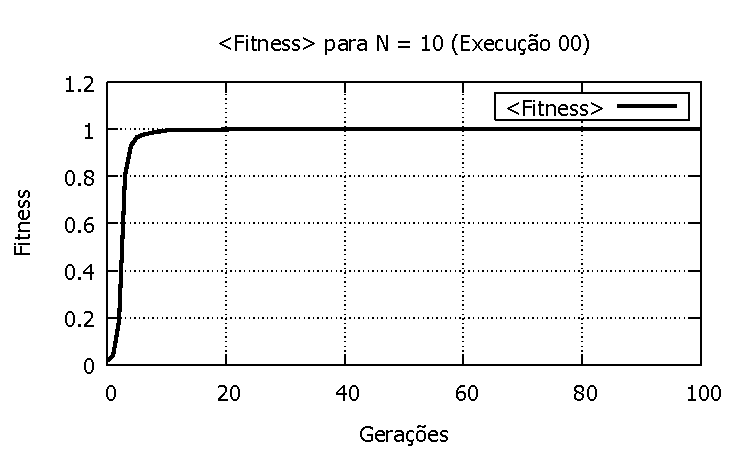
\includegraphics{figs/resultados/fitnessGrad/N10_00_fitness.pdf}
			\caption{Comportamento do \textsl{fitness} $f_i = e^{-\lambda \| \nabla \rho_i \|^2}$ para N = 10. Na primeira geração o melhor \textit{fitness} é pequeno, aproximadamente 0,1, cresce rapidamente e a partir da décima geração está próximo de 1.}
		\label{fig:compFitnessTipo1N10}
	\end{figure}
	
	O próximo passo foi verificar o comportamento de $\rho$, o Quociente de Rayleigh, e, especificamente, sua convergência para o menor autovalor $E_0$. Ainda conforme \cite{metodo2004}, obteríamos uma curva semelhante à da figura \ref{fig:compFitnessTipo1N10}, mas invertida, ou seja, os primeiros valores de $\rho$ seriam grandes e, rapidamente, diminuiriam até haver convergência para o autovalor mínimo. Na figura \ref{fig:rho_N10} há um exemplo.	Os gráficos exibem os valores de $\rho$ para a mesma execução apresentada na figura \ref{fig:compFitnessTipo1N10}. Note no primeiro gráfico que até a geração 20 o quociente $\rho$ teve caráter oscilatório e, então, aparentemente estabilizou-se entre 6 e 8, valores muito superiores ao autovalor mínimo para essa matriz, $E_0 = 0,38675$. Entretanto, ainda no primeiro gráfico, observa-se que há uma tendência de queda do $\rho$ entre as gerações 40 e 50 e, portanto, existiria a possibilidade do algoritmo convergir para $E_0$. Porém, para esse exemplo especificamente, isso não aconteceu, como pode ser visto no segundo gráfico da figura \ref{fig:rho_N10}. Para garantir a estabilidade, o programa foi executado até a geração 400.000, e o valor médio obtido foi $<\rho> = 6,572898$. Para nossa surpresa, além do valor obtido de $<\rho>$ não ser o mínimo, ele não é um valor qualquer, mas corresponde, com erro menor que $0,00002\%$, ao quarto autovalor da matriz, $E_3 = 6,572897$. Um gráfico expandido dessa execução está na figura \ref{fig:rho_N10_completa} da página \pageref{fig:rho_N10_completa}. Pensamos, então, que poderia haver algo de errado com o nosso programa. 
	
	\begin{figure}[htbp]
		\centering
			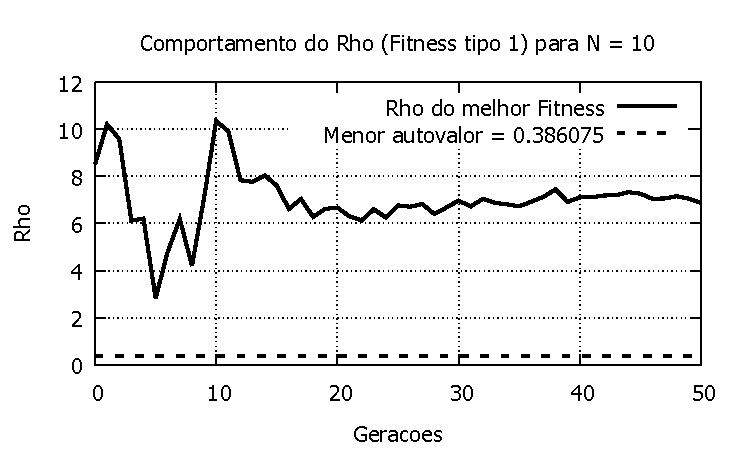
\includegraphics[width=0.40\textwidth]{figs/resultados/rho_N10_g50.pdf}
			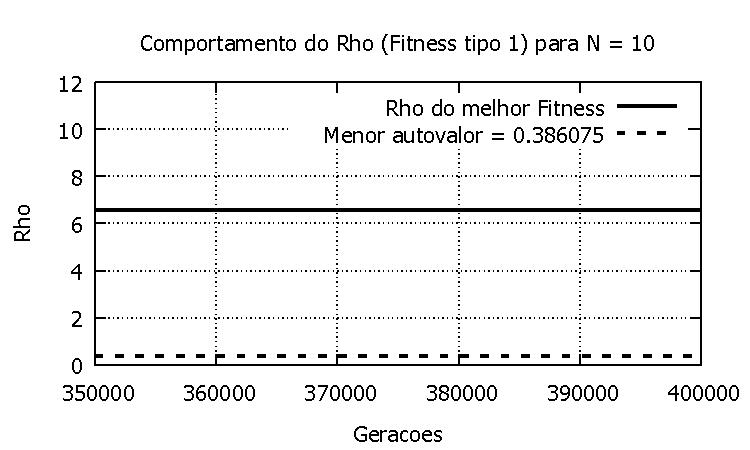
\includegraphics[width=0.40\textwidth]{figs/resultados/rho_N10_g400000.pdf}
		\caption{Comportamento de $\rho$ (Quociente de Rayleigh) para uma matriz de Coope$-$Sabo de ordem 10.}
		\label{fig:rho_N10}
	\end{figure}
	
	\newpage
	\begin{landscape}
	\begin{figure}[p]
		\centering
			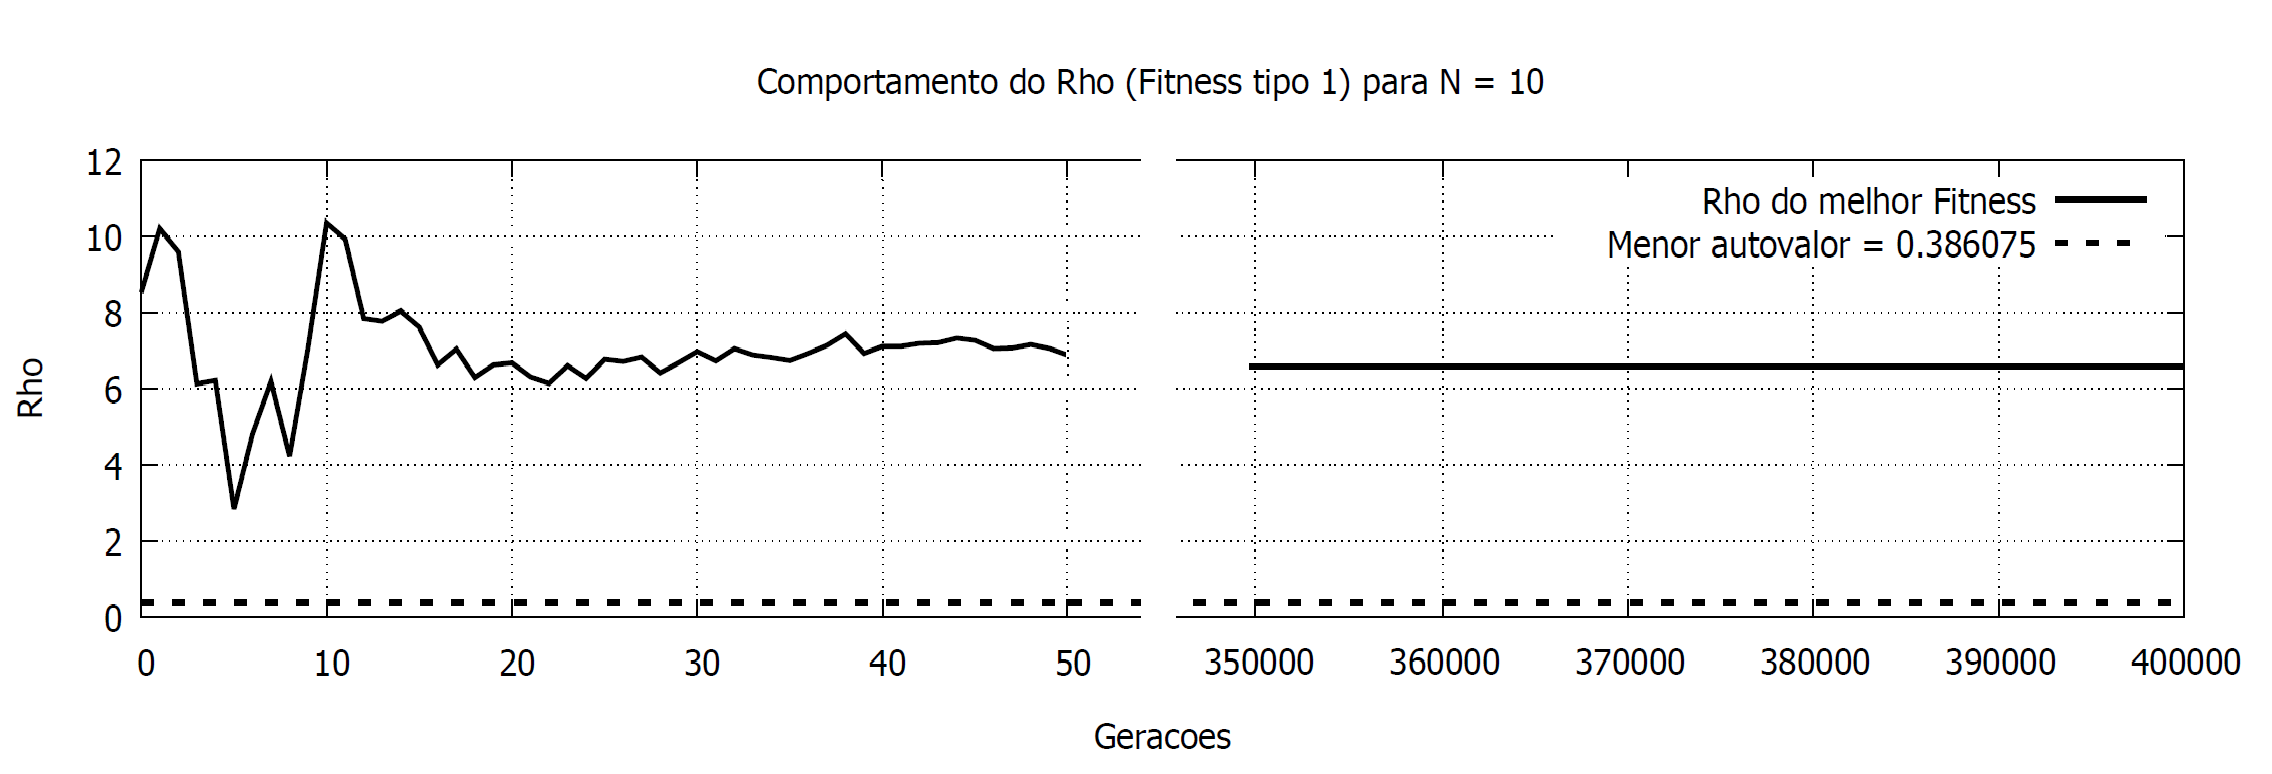
\includegraphics[width=1.3\textwidth]{figs/resultados/rho_N10.png}
		\caption{Comportamento de $\rho$ (Quociente de Rayleigh) para uma matriz de Coope$-$Sabo de ordem 10.}
		\label{fig:rho_N10_completa}
	\end{figure}
	\end{landscape}
	\newpage
			
	Após esses resultados preliminares executamos uma validação cuidadosa do programa, testando cada uma de suas quase 2500 linhas e comparando os resultados das operações e cálculos com os softwares Excel \cite{excel} e SciLab \cite{scilab}. A hipótese era a de que erros numéricos, principalmente nas funções de álgebra linear e nos operadores genéticos, pudessem ter levado ao comportamento incorreto da não convergência para o menor autovalor. De fato alguns erros foram encontrados.
	
	Discutiremos a seguir os testes com a versão corrigida do programa e exibidos nas figuras \ref{fig:execucoes_N10}, \ref{fig:execucoes_N20}, \ref{fig:execucoes_N30} e \ref{fig:execucoes_N40}. Visando brevidade, apresentaremos dados para matrizes de Coope\-Sabo de ordem 10, 20, 30 e 40 apenas, sem perda de generalidade. Foram cinco execuções para cada matriz, até a geração 400.000, gerando sempre dois gráficos, um do \textit{fitness} médio (<\textit{fitness}>) e outro do Quociente de Rayleigh médio (<$\rho$>), ambos em função do número de gerações, e dando ênfase às primeiras 100 gerações. Essas escolhas, número máximo da geração e uso de médias sobre cada população, visaram garantir, respectivamente, a convergência genética e boa precisão. A exibição de apenas as primeiras 100 gerações tem como objetivo olhar em detalhe (com \textit{zoom}) o período em que o \textit{crossover} tem mais peso, ou seja, onde há geralmente os saltos no espaço de soluções de um Algoritmo Genético. Em todos os gráficos de $<\rho>$ há indicado nas legendas o autovalor mínimo $E_0$ e o autovalor obtido após as 400.000 gerações ($E_{obtido}$). Na tabela \ref{tab:autovalores10a40} há a lista de todos os autovalores. Por exemplo, para uma matriz de ordem $N = 10$, o menor autovalor é $E_0 = $0,386075, e o quinto autovalor para $N = 30$ é $E_4$ = 8,450274.
	
	Comecemos a discussão com o que foi encontrado em todas as execuções. Em qualquer gráfico do \textit{fitness} observa-se estabilidade do comportamento conforme esperado pelo método: no início seu valor é baixo, próximo de zero, cresce rapidamente nas primeiras gerações e fica estável próximo de $<fitness> = 1$. Com relação ao $\rho$, há sempre oscilações, sejam pequenas variações em torno de uma clara linha de tendência, como na execução 02 para N = 10, ou grandes saltos, como nas execuções 05 de N = 20 e 05 de N = 30. Novamente, o menor autovalor não foi obtido em nenhuma execução, contradizendo os resultados de \cite{metodo2004}, mas, por outro lado, o algoritmo sempre encontrou algum autovalor.
	
	De fato, verificando os dados da tabela \ref{tab:execucoes10a40}, concluímos que tais valores não devem ser coincidência. Para todas as execuções o \textit{fitness} médio chegou ao valor máximo ($<f> = 1,000000$). As médias de $\rho$ sobre todos os indivíduos da última população possuem baixo desvio padrão ($\sigma$ < 0,0001), indicando que eles são muito parecidos entre si e que o algoritmo atingiu a convergência genética. Ou seja, não há variabilidade genética suficiente na população para alterar o rumo da busca de modo a atingir o menor autovalor, ou o mínimo global. Portanto, o algoritmo chegou em um mínimo local, corroborado pelos baixos erros relativos de $<\rho>$ quando comparado com o autovalor mais próximo. Por exemplo, para N = 30, execução 4,  $<\rho>$ = 40,772447, correspondendo, com erro relativo absoluno menor que $0,001\%$, ao vigésimo primeiro autovalor, $E_{20} = 40,772850$. Apesar das evidências descritas acima, até esse ponto ainda há dúvidas sobre a validade do nosso programa e, obviamente, dos resultados produzidos. Então, buscamos embasamento mais rigoroso.

De acordo com \cite{metodo2004}, se algum $C_i$, em algum momento, é o autovetor fundamental (associado ao menor autovalor), o $\nabla \rho$ é nulo. Com o \textit{fitness} da equação \eqref{eq:fitnessGrad2} os autores afirmam que ``\textit{Claramente, $f_i \rightarrow 1$ quando $\nabla \rho_i \rightarrow 0$, sinalizando que a evolução atingiu o verdadeiro autovetor fundamental de $H$ em $C_i$}''\footnote{Tradução livre de ``\textit{Clearly, $f_i \rightarrow 1$, as $\nabla \rho_i \rightarrow 0$, signalling that the evolution has hit the true ground state eigenvector of $H$ in the vector $C_i$}''.}. Há duas relações distintas de causalidade nessa frase, e acreditamos que nelas residam a explicação dos resultados obtidos por nós até agora.

A primeira relação de causalidade refere-se à afirmação ``\textit{$f_i \rightarrow 1$ quando $\nabla \rho_i \rightarrow 0$}'', que está absolutamente correta. Retomando a seção \ref{cap:metodologia}, o \textit{fitness} definido pela equação \ref{eq:fitnessGrad2} é limitado no intervalo (0,1] e, como $\lambda > 0$, só chega ao seu valor máximo quando $\nabla \rho_i = 0$. Em outras palavras, $\nabla \rho_i \rightarrow 0$ implica $f_i \rightarrow 1$.

Na afirmação ``(...) \textit{sinalizando que a evolução atingiu o verdadeiro autovetor fundamental de $H$ em $C_i$}'' reside a segunda relação de causalidade que, apesar de sutil, é muito poderosa:

\begin{equation}\label{eq:afirmacaoErrada}
	\mbox{Se } f_i \rightarrow 1\mbox{, } C_i = C_0.
\end{equation}

Ou seja, sempre que algum indivíduo $C_i$, de qualquer população, possuir \textit{fitness} muito próximo de 1, isso implica que, além de ter uma excelente ``nota'', ele, ainda por cima, é um vetor especial, o autovetor fundamental $C_0$. Portanto, possui autovalor associado $E_0$, o autovalor mínimo (conforme equação \ref{eq:rho_eh_E}). Grosso modo, $f_i(C_i) = 1$ implica que $C_i = C_0$ e que podemos obter $E_0(C_0)$:

\begin{equation}\label{eq:causalidadeErrada}
	f_i(C_i) = 1 \rightarrow C_i = C_0 \rightarrow E_0(C_0).
\end{equation}

As relações de causa e efeito da equação acima estão erradas. Em sua obra clássica sobre o problema de autovalores em matrizes simétricas, \cite{Parlett1998} abre o capítulo introdutório frisando que ``\textit{em muitos lugares no livro, é feita referência a fatos mais ou menos bem conhecidos sobre a teoria de matrizes}''\footnote{Tradução livre de ``\textit{At many places in the book, reference is made to more or less well known facts from matrix theory}''.}. Conforme já dito no capítulo \ref{cap:algebra}, um desses fatos diz que $\rho(\mbox{\textit{u}})$ é estacionário, ou seja, $\nabla \rho(\mbox{\textit{u}}) = 0$, apenas se o vetor \textit{u} é um autovetor $w$ de $HC = EC$. Consequentemente, o encadeamento correto se apresenta como:

\begin{equation}\label{eq:causalidadeCorreta}
	C_i \mbox{ é um autovetor} \rightarrow \nabla \rho(C_i) = 0 \rightarrow f_i = 1.
\end{equation}
	
Então, se $f_i = 1$, o máximo que podemos concluir é que $C_i$ é \textit{algum} autovetor, e não necessariamente \textit{o} autovetor fundamental. Ao fim de todos os nossos testes o \textit{fitness} médio foi <\textit{f}> = 1, a população final era composta por autovetores e foi possível, com boa precisão, obter os autovalores relacionados (não necessariamente o autovalor mínimo). Nossos dados confirmam a matemática e, assim, acreditamos que nosso programa não contém erros.

Apesar de não chegar ao mínimo, o método pode ser utilizado de maneira exploratória com relativa facilidade, bastando extrair $\rho$ sempre que $f_i \rightarrow 1$ e $\nabla \rho \rightarrow 0$. 

Resta a dúvida: afinal, como o autovalor mínimo foi obtido com o \textit{fitness} definido pela equação \ref{eq:fitnessGrad2}? Não sabemos. Esse \textit{fitness} foi utilizado não só em \cite{metodo2004}, mas também em \cite{metodo2006}, \cite{metodo2008} e \cite{metodo2009}, seguindo exatamente o argumento resumido pela equação \ref{eq:causalidadeErrada}. Não identificamos nada nesses quatro artigos que pudesse levar à resposta. Seguimos o estudo com uma nova definição do \textit{fitness} encontrada em \cite{metodo2011}.

\begin{figure}[phtb]
\centering
  \begin{tabular}{@{}cc@{}}
    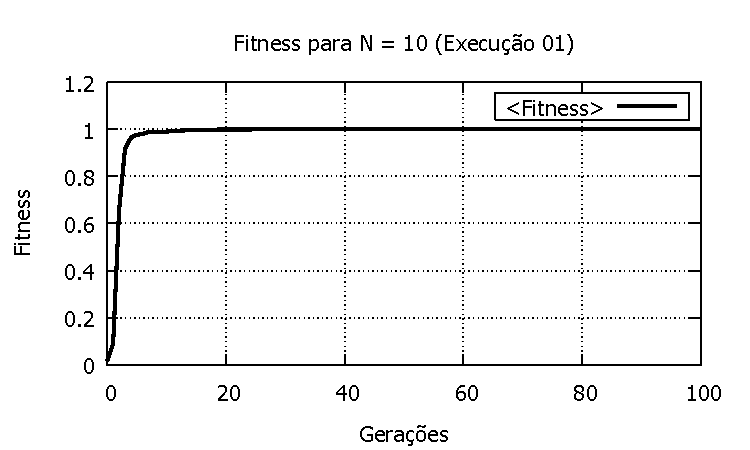
\includegraphics[width=.40\textwidth]{figs/resultados/fitnessGrad/N10_01_fitness.pdf} &
    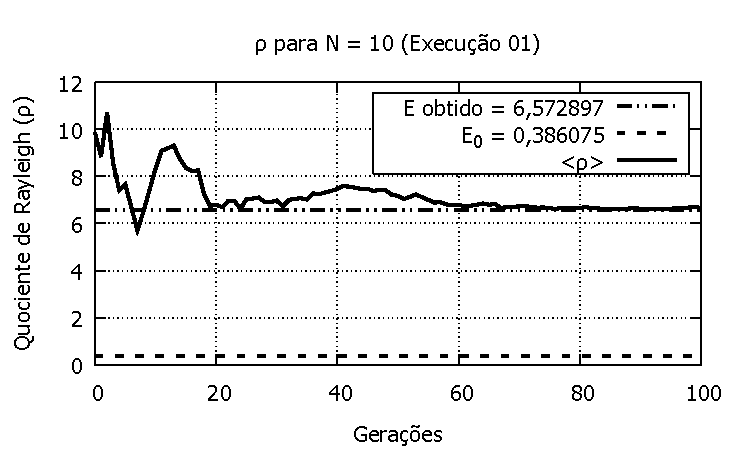
\includegraphics[width=.40\textwidth]{figs/resultados/fitnessGrad/N10_01_rho.pdf}   \\
		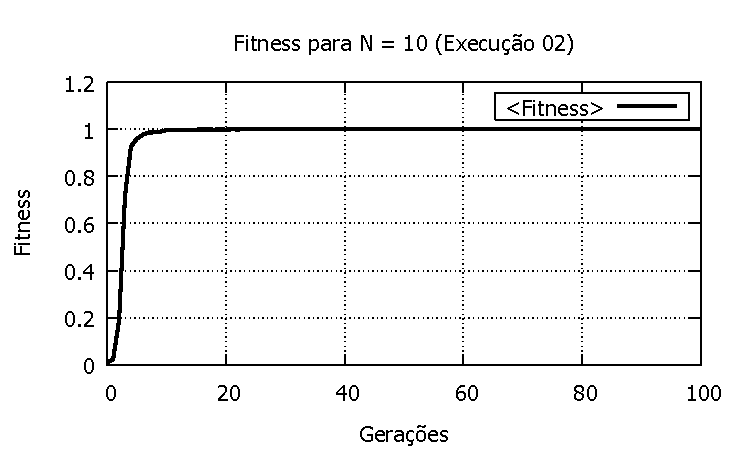
\includegraphics[width=.40\textwidth]{figs/resultados/fitnessGrad/N10_02_fitness.pdf} &
    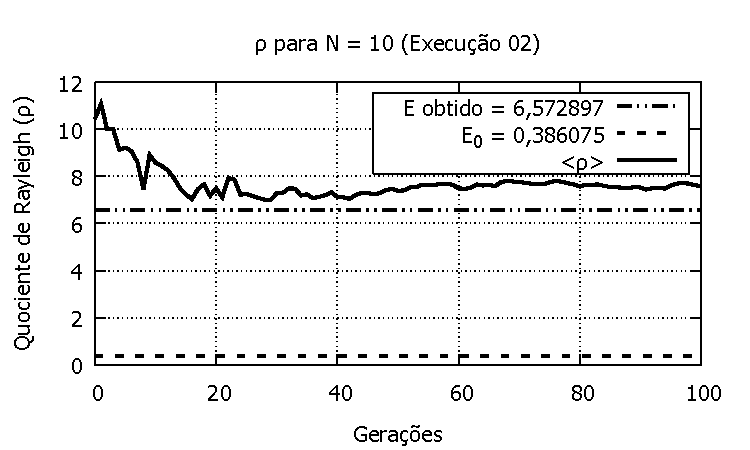
\includegraphics[width=.40\textwidth]{figs/resultados/fitnessGrad/N10_02_rho.pdf}   \\
		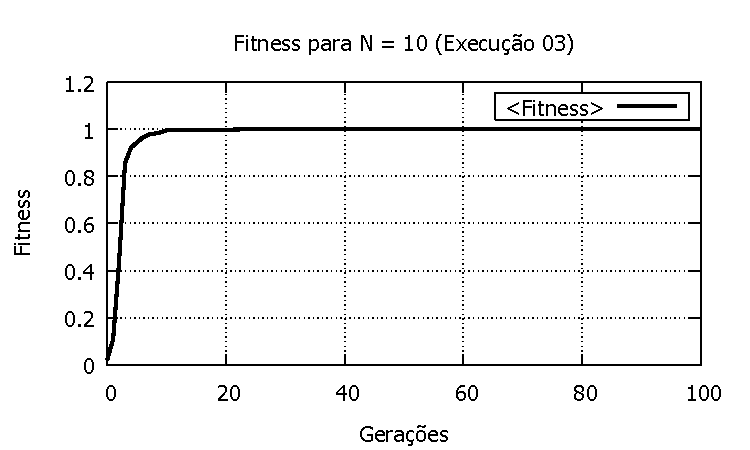
\includegraphics[width=.40\textwidth]{figs/resultados/fitnessGrad/N10_03_fitness.pdf} &
    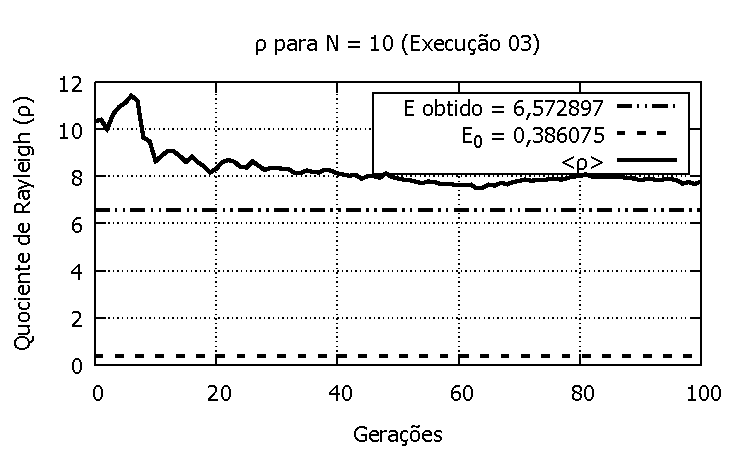
\includegraphics[width=.40\textwidth]{figs/resultados/fitnessGrad/N10_03_rho.pdf}   \\
		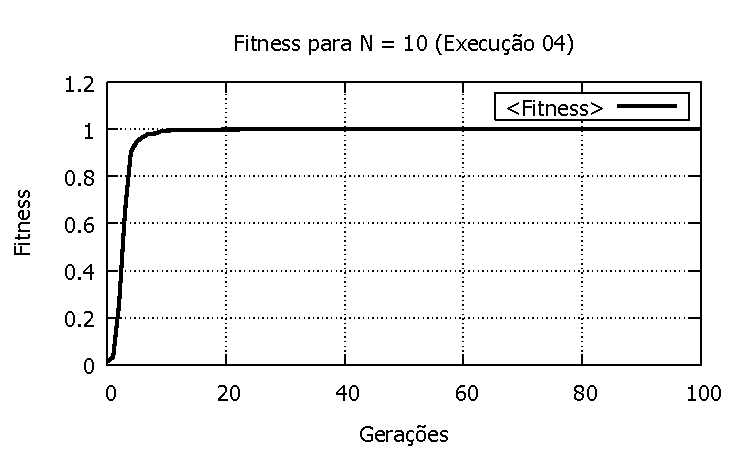
\includegraphics[width=.40\textwidth]{figs/resultados/fitnessGrad/N10_04_fitness.pdf} &
    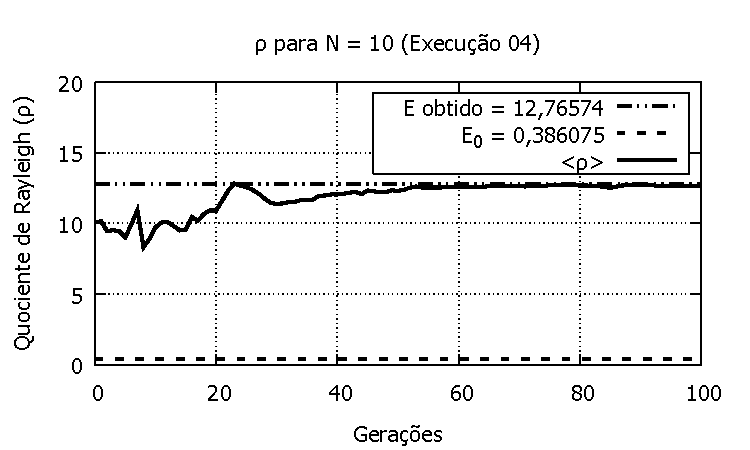
\includegraphics[width=.40\textwidth]{figs/resultados/fitnessGrad/N10_04_rho.pdf}   \\
		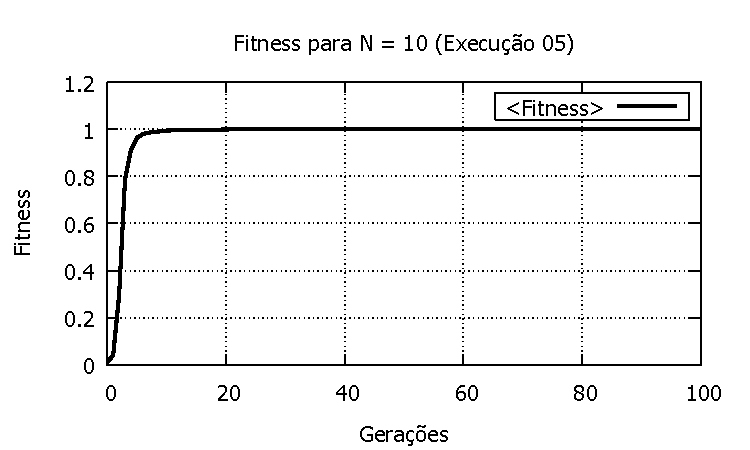
\includegraphics[width=.40\textwidth]{figs/resultados/fitnessGrad/N10_05_fitness.pdf} &
    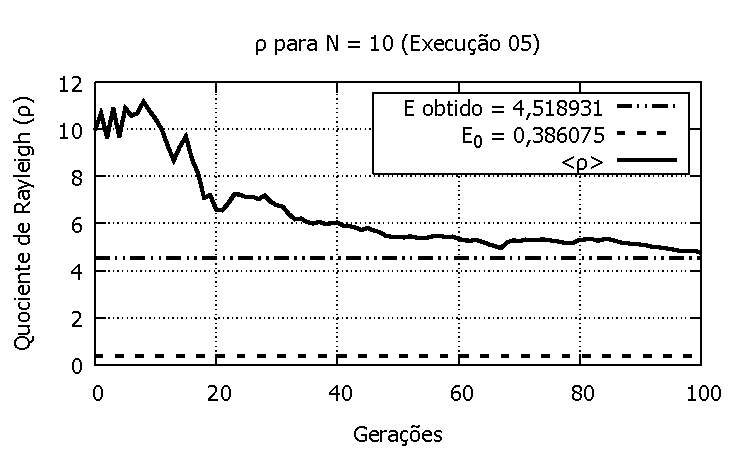
\includegraphics[width=.40\textwidth]{figs/resultados/fitnessGrad/N10_05_rho.pdf}
    %\multicolumn{2}{c}{\includegraphics[width=.23\textwidth]{example-image-a}}
  \end{tabular}
  \caption{Execuções N = 10.}
	\label{fig:execucoes_N10}
\end{figure}

\begin{figure}[phtb]
\centering
  \begin{tabular}{@{}cc@{}}
    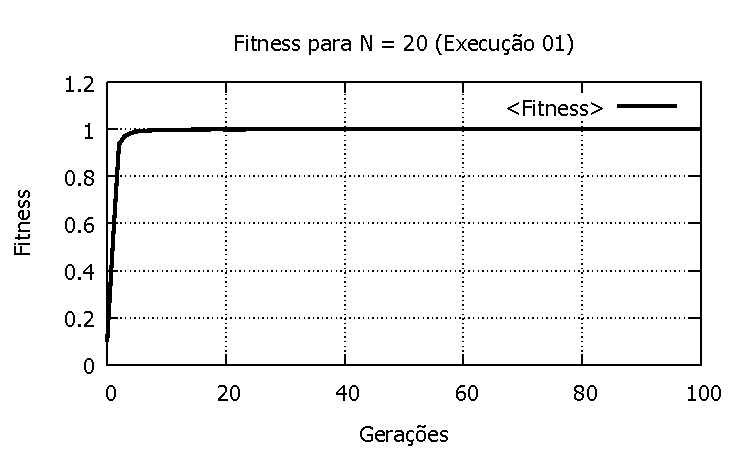
\includegraphics[width=.40\textwidth]{figs/resultados/fitnessGrad/N20_01_fitness.pdf} &
    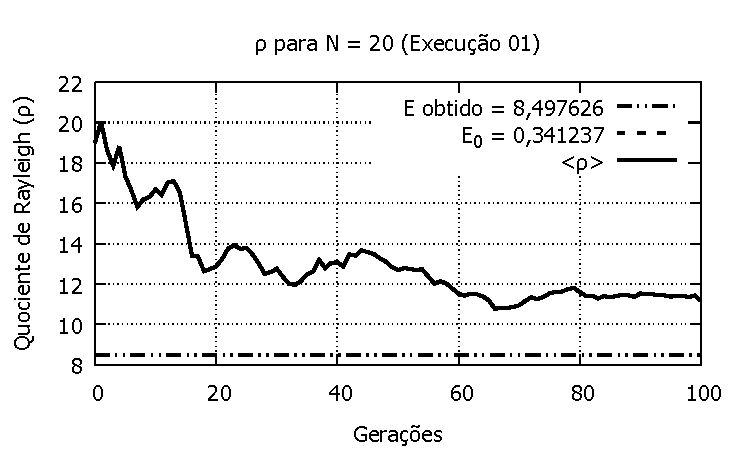
\includegraphics[width=.40\textwidth]{figs/resultados/fitnessGrad/N20_01_rho.pdf}   \\
		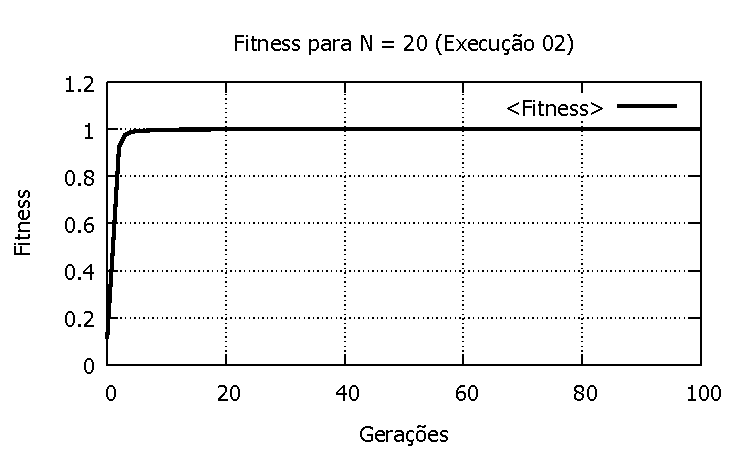
\includegraphics[width=.40\textwidth]{figs/resultados/fitnessGrad/N20_02_fitness.pdf} &
    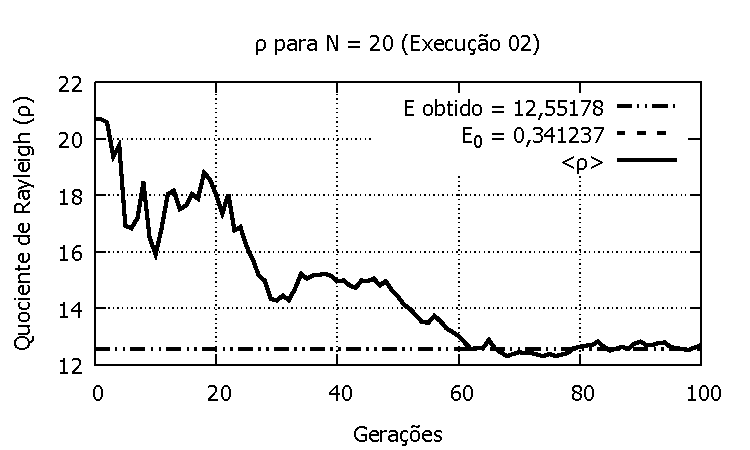
\includegraphics[width=.40\textwidth]{figs/resultados/fitnessGrad/N20_02_rho.pdf}   \\
		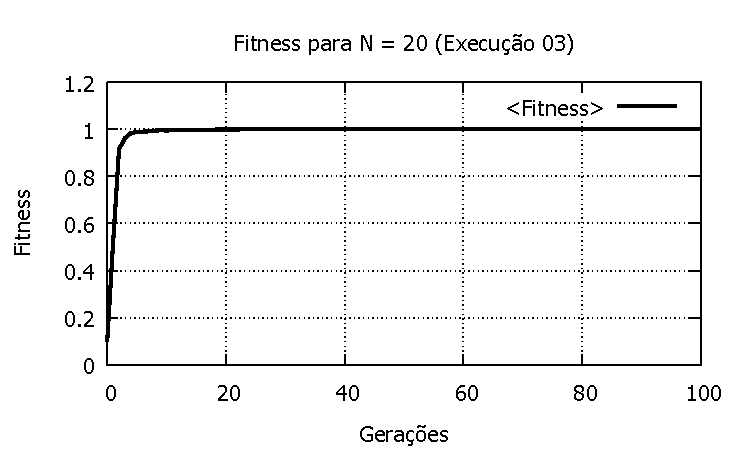
\includegraphics[width=.40\textwidth]{figs/resultados/fitnessGrad/N20_03_fitness.pdf} &
    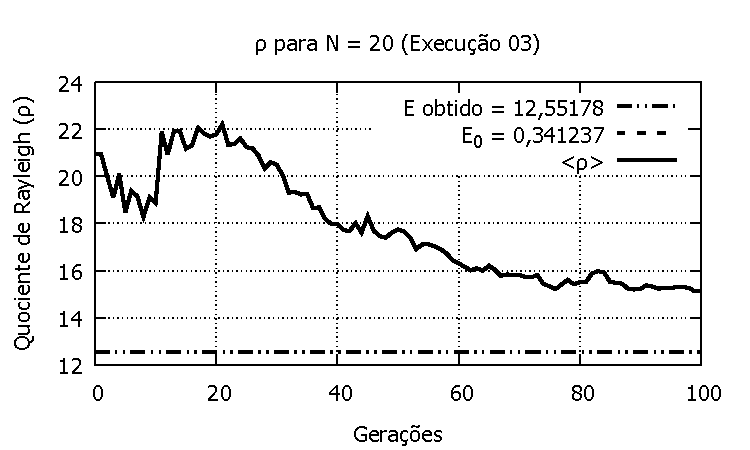
\includegraphics[width=.40\textwidth]{figs/resultados/fitnessGrad/N20_03_rho.pdf}   \\
		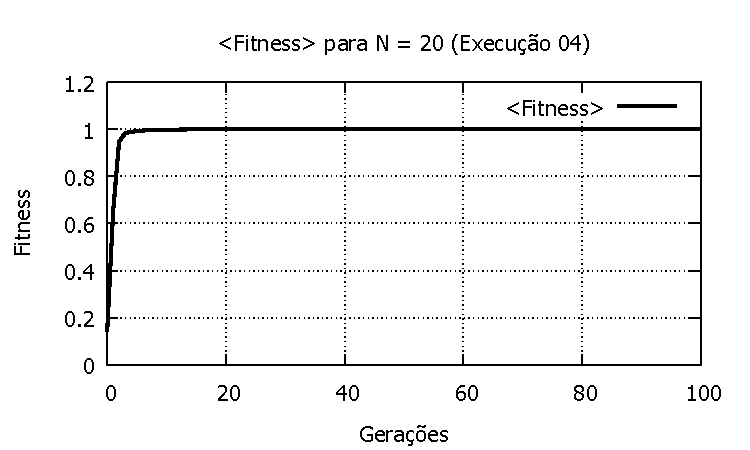
\includegraphics[width=.40\textwidth]{figs/resultados/fitnessGrad/N20_04_fitness.pdf} &
    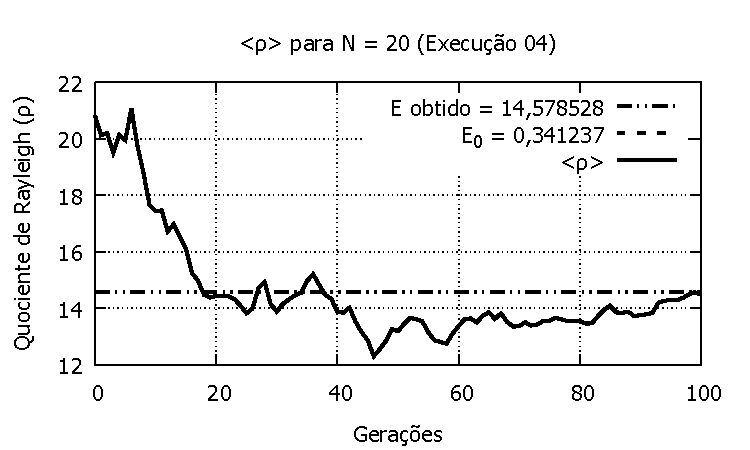
\includegraphics[width=.40\textwidth]{figs/resultados/fitnessGrad/N20_04_rho.pdf}   \\
		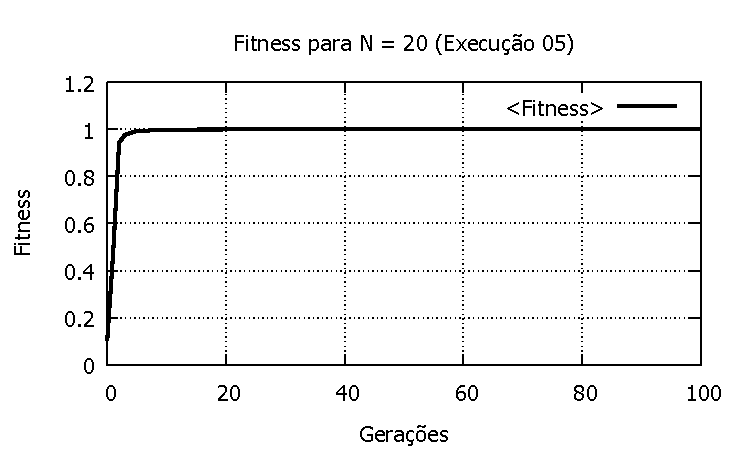
\includegraphics[width=.40\textwidth]{figs/resultados/fitnessGrad/N20_05_fitness.pdf} &
    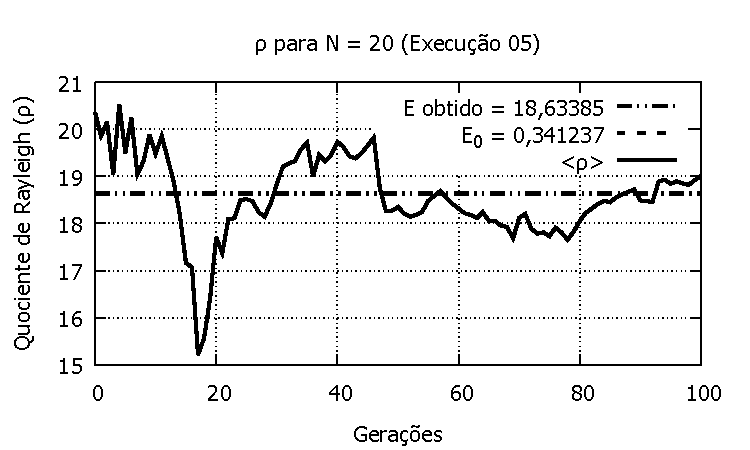
\includegraphics[width=.40\textwidth]{figs/resultados/fitnessGrad/N20_05_rho.pdf}
    %\multicolumn{2}{c}{\includegraphics[width=.23\textwidth]{example-image-a}}
  \end{tabular}
  \caption{Execuções N = 20.}
	\label{fig:execucoes_N20}
\end{figure}

\begin{figure}[phtb]
\centering
  \begin{tabular}{@{}cc@{}}
    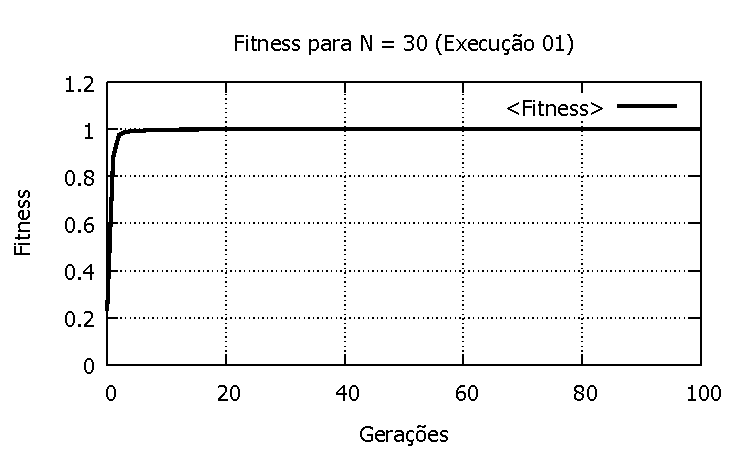
\includegraphics[width=.40\textwidth]{figs/resultados/fitnessGrad/N30_01_fitness.pdf} &
    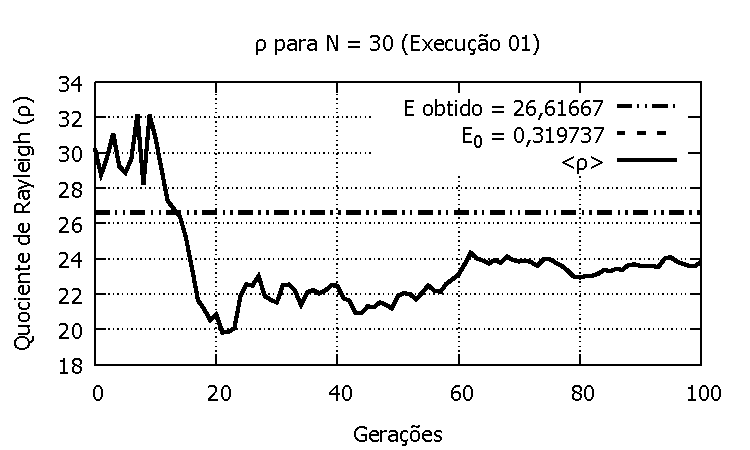
\includegraphics[width=.40\textwidth]{figs/resultados/fitnessGrad/N30_01_rho.pdf}   \\
		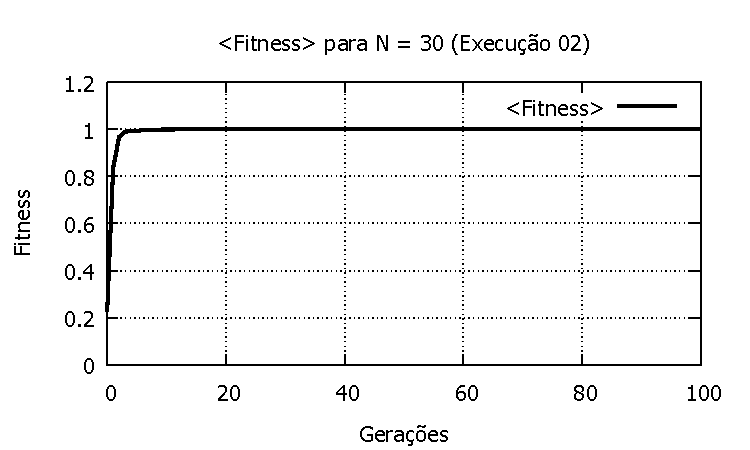
\includegraphics[width=.40\textwidth]{figs/resultados/fitnessGrad/N30_02_fitness.pdf} &
    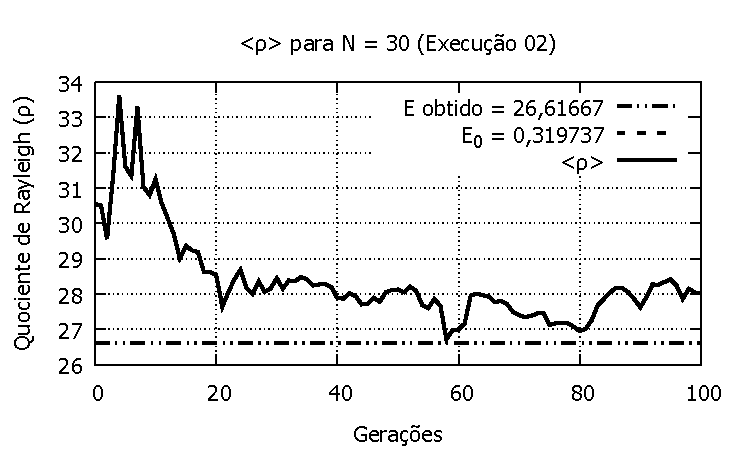
\includegraphics[width=.40\textwidth]{figs/resultados/fitnessGrad/N30_02_rho.pdf}   \\
		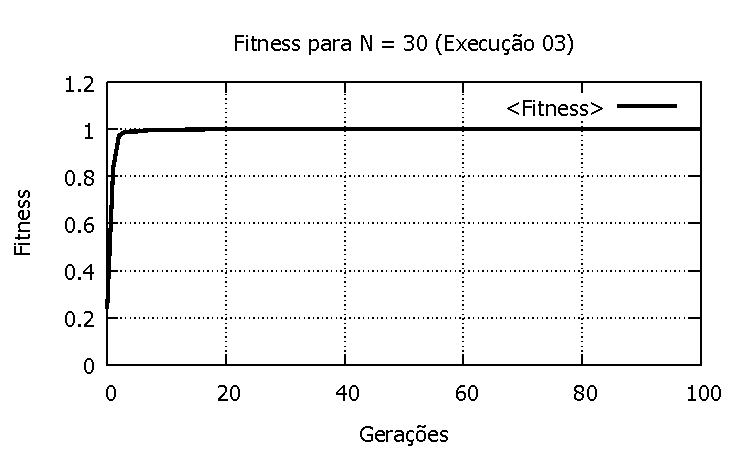
\includegraphics[width=.40\textwidth]{figs/resultados/fitnessGrad/N30_03_fitness.pdf} &
    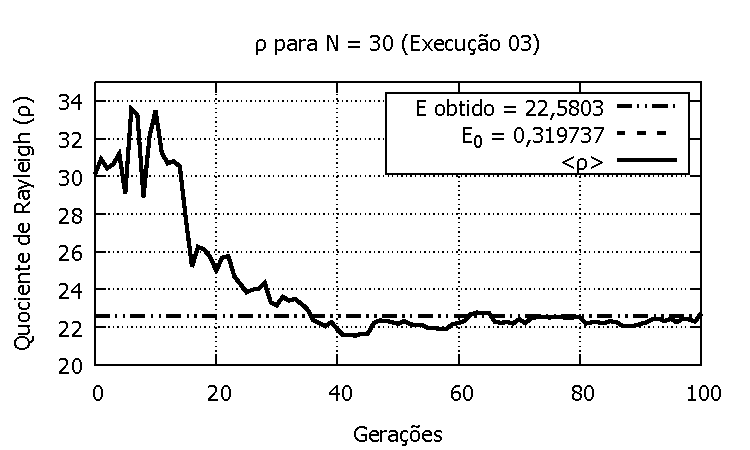
\includegraphics[width=.40\textwidth]{figs/resultados/fitnessGrad/N30_03_rho.pdf}   \\
		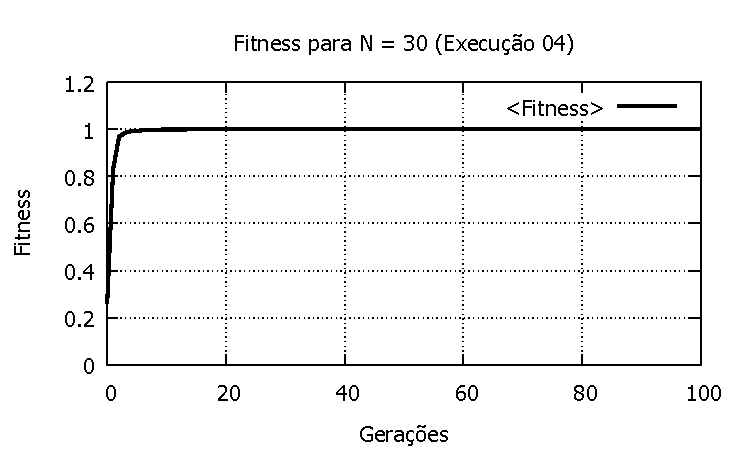
\includegraphics[width=.40\textwidth]{figs/resultados/fitnessGrad/N30_04_fitness.pdf} &
    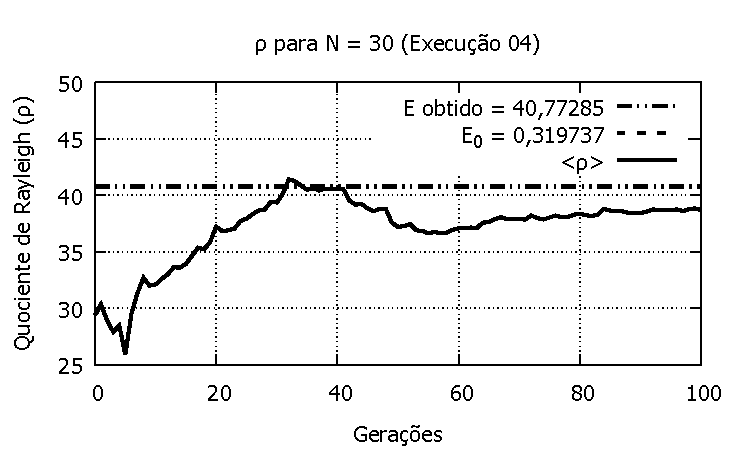
\includegraphics[width=.40\textwidth]{figs/resultados/fitnessGrad/N30_04_rho.pdf}   \\
		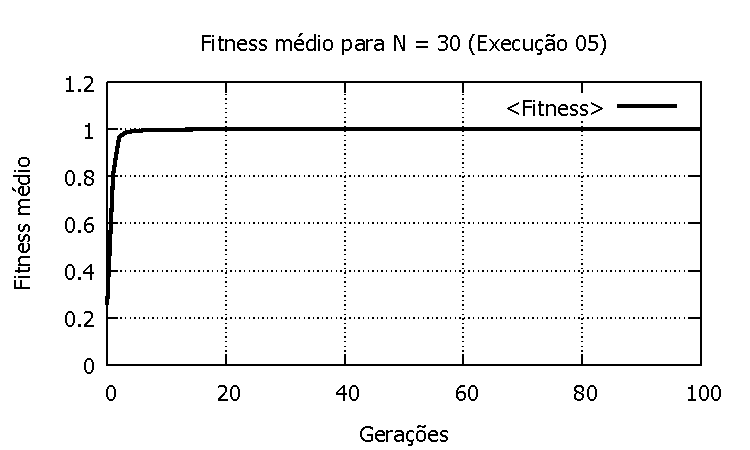
\includegraphics[width=.40\textwidth]{figs/resultados/fitnessGrad/N30_05_fitness.pdf} &
    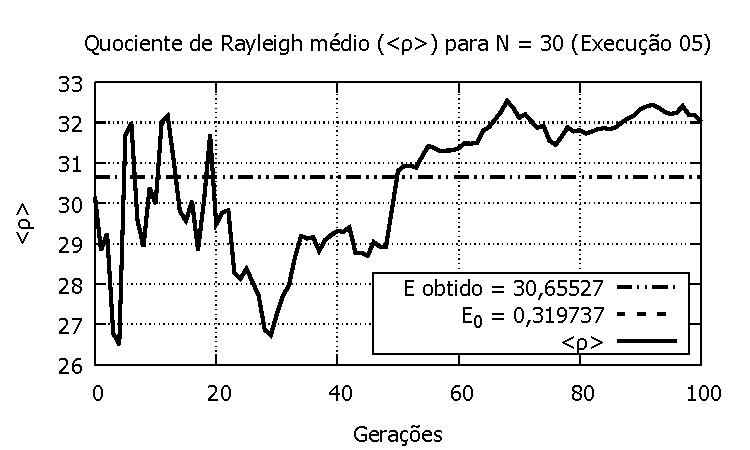
\includegraphics[width=.40\textwidth]{figs/resultados/fitnessGrad/N30_05_rho.pdf}
    %\multicolumn{2}{c}{\includegraphics[width=.23\textwidth]{example-image-a}}
  \end{tabular}
  \caption{Execuções N = 30.}
	\label{fig:execucoes_N30}
\end{figure}

\begin{figure}[phtb]
\centering
  \begin{tabular}{@{}cc@{}}
    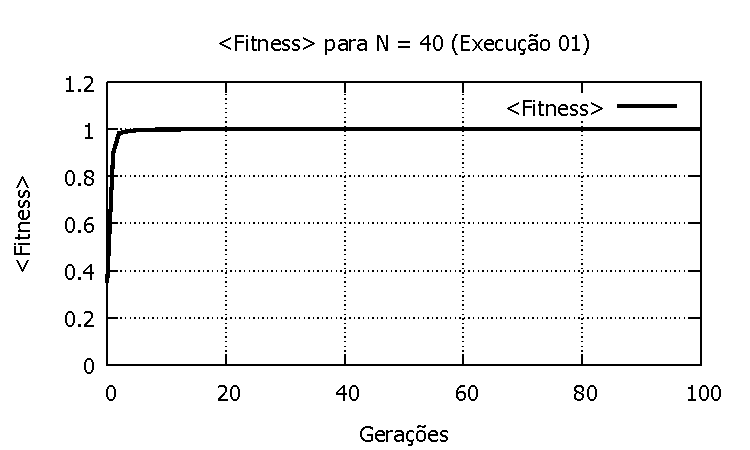
\includegraphics[width=.40\textwidth]{figs/resultados/fitnessGrad/N40_01_fitness.pdf} &
    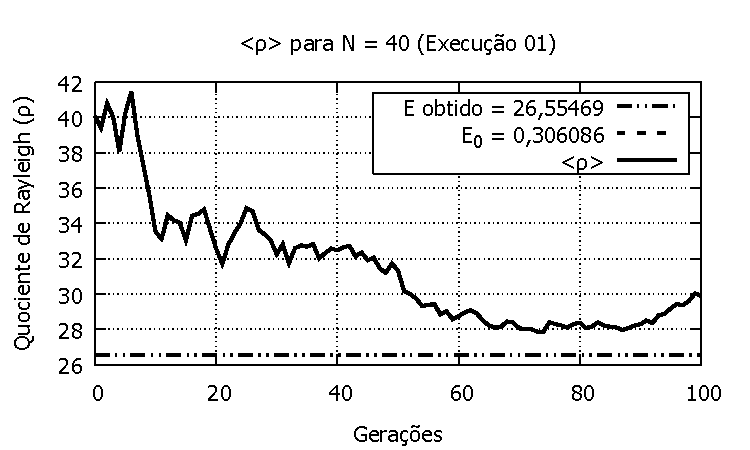
\includegraphics[width=.40\textwidth]{figs/resultados/fitnessGrad/N40_01_rho.pdf}   \\
		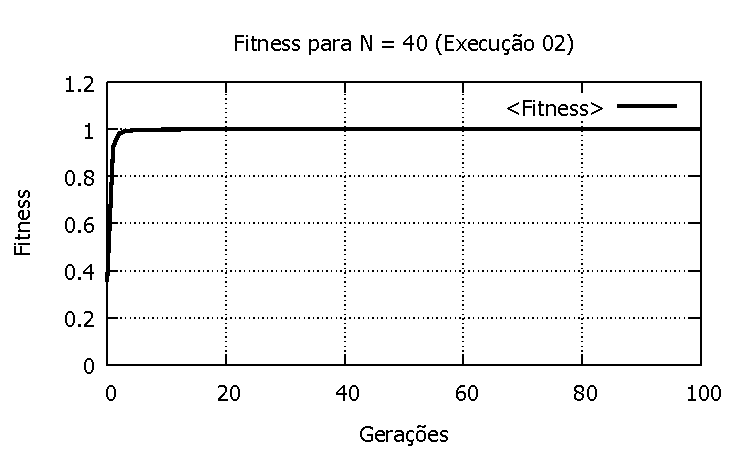
\includegraphics[width=.40\textwidth]{figs/resultados/fitnessGrad/N40_02_fitness.pdf} &
    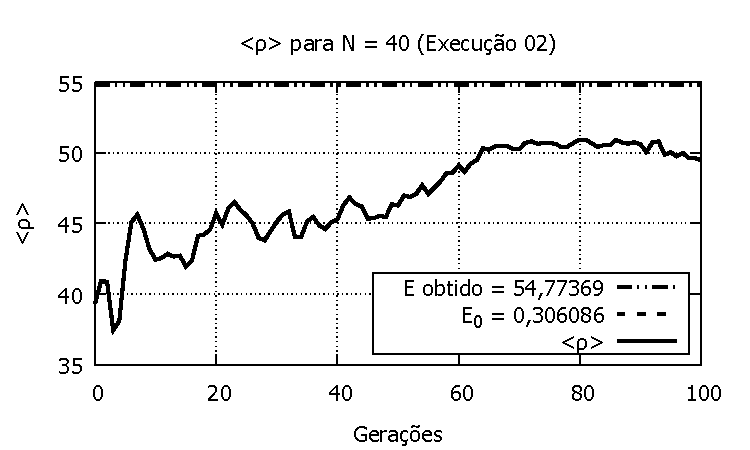
\includegraphics[width=.40\textwidth]{figs/resultados/fitnessGrad/N40_02_rho.pdf}   \\
		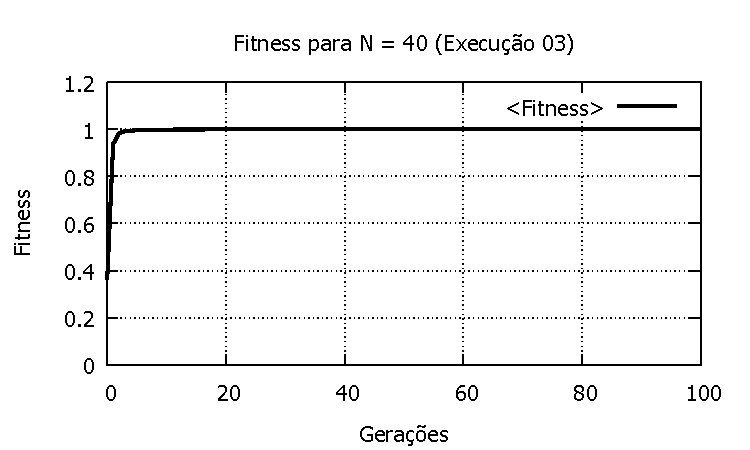
\includegraphics[width=.40\textwidth]{figs/resultados/fitnessGrad/N40_03_fitness.pdf} &
    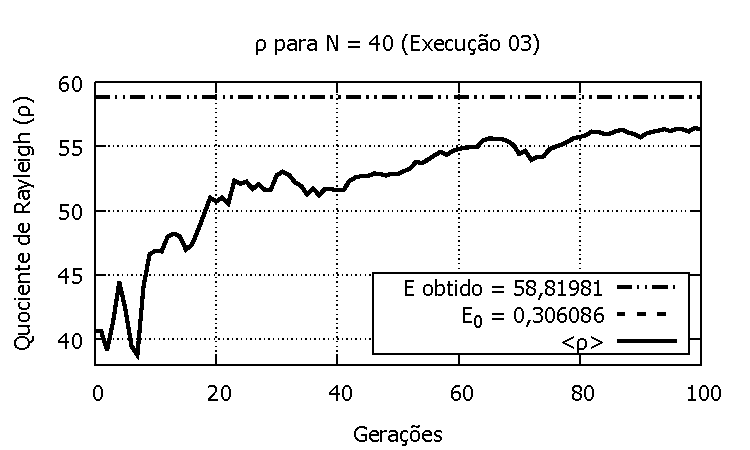
\includegraphics[width=.40\textwidth]{figs/resultados/fitnessGrad/N40_03_rho.pdf}   \\
		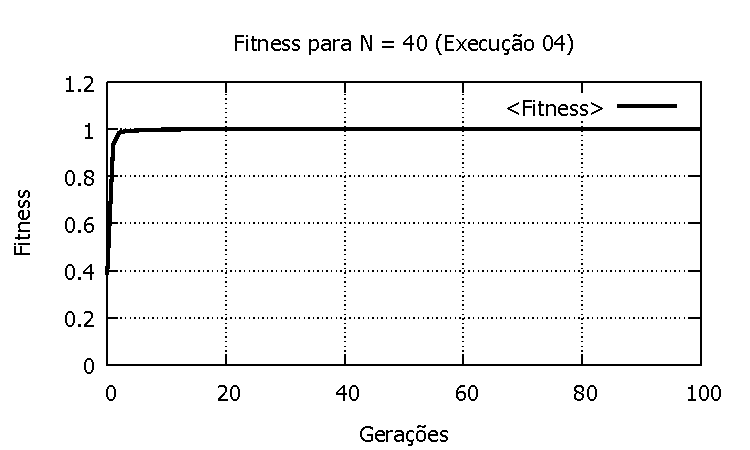
\includegraphics[width=.40\textwidth]{figs/resultados/fitnessGrad/N40_04_fitness.pdf} &
    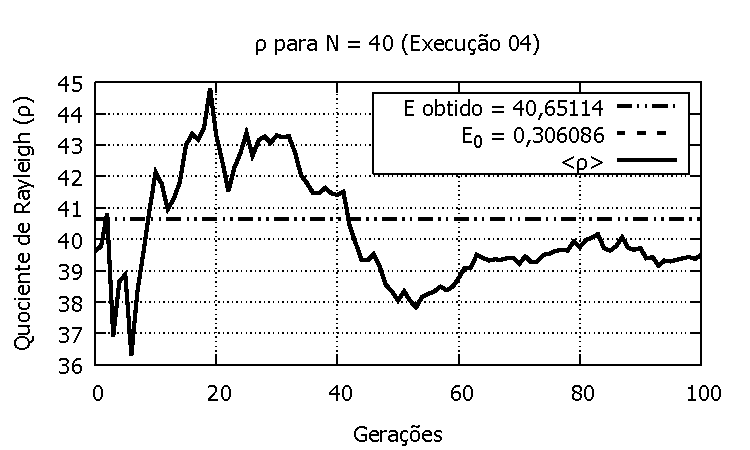
\includegraphics[width=.40\textwidth]{figs/resultados/fitnessGrad/N40_04_rho.pdf}   \\
		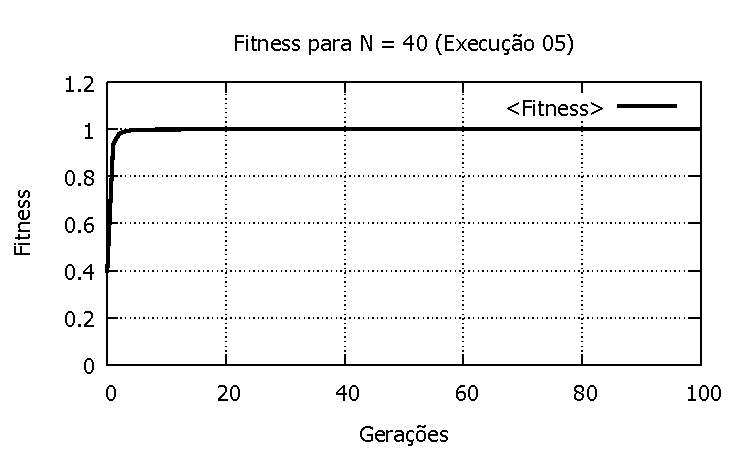
\includegraphics[width=.40\textwidth]{figs/resultados/fitnessGrad/N40_05_fitness.pdf} &
    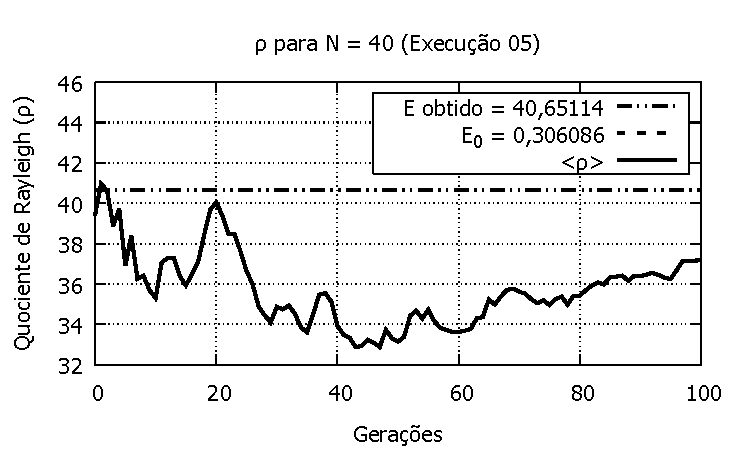
\includegraphics[width=.40\textwidth]{figs/resultados/fitnessGrad/N40_05_rho.pdf}
    %\multicolumn{2}{c}{\includegraphics[width=.23\textwidth]{example-image-a}}
  \end{tabular}
  \caption{Execuções N = 40.}
	\label{fig:execucoes_N40}
\end{figure}

\begin{landscape}
\begin{center}
\begin{table}[htbp]
\caption{Execuções para matrizes de Coope$-$Sabo.}
\label{tab:execucoes10a40}
% Table generated by Excel2LaTeX from sheet 'Plan1 (2)'
\begin{tabular}{cccccccccc}
\hline \hline
   \textbf{N} & \textbf{Execução} & \textbf{Semente} & \textbf{$\lambda$} & \textbf{<\textit{Fitness}>} & \textbf{<$\rho$>} & \textbf{$\sigma$} & \textbf{\# autovalor} & \textbf{Autovalor} & \textbf{Erro relativo} \\
\hline \hline
        10 &          0 & 1445738835 &   0,128788 &   1,000000 &   2,461122 &   0,000023 &          1 &   2,461056 &    0,003\% \\
\hline
        10 &          1 & 1445780626 &   0,128788 &   1,000000 &   6,572898 &   0,000013 &          3 &   6,572897 &  0,00001\% \\
\hline
        10 &          2 & 1445780762 &   0,128788 &   1,000000 &   6,572883 &   0,000015 &          3 &   6,572897 &  -0,0002\% \\
\hline
        10 &          3 & 1445780907 &   0,128788 &   1,000000 &   6,572910 &   0,000016 &          3 &   6,572897 &   0,0002\% \\
\hline
        10 &          4 & 1445781049 &   0,128788 &   1,000000 &  12,765701 &   0,000016 &          6 &  12,765740 &  -0,0003\% \\
\hline
        10 &          5 & 1445781195 &   0,128788 &   1,000000 &   4,518952 &   0,000012 &          2 &   4,518931 &   0,0005\% \\
\hline
        20 &          1 & 1445795292 &   0,026665 &   1,000000 &   8,498192 &   0,000052 &          4 &   8,497626 &    0,007\% \\
\hline
        20 &          2 & 1445795501 &   0,026665 &   1,000000 &  12,551830 &   0,000018 &          6 &  12,551780 &   0,0004\% \\
\hline
        20 &          3 & 1445795718 &   0,026665 &   1,000000 &  12,551878 &   0,000020 &          6 &  12,551780 &   0,0008\% \\
\hline
        20 &          4 & 1445795953 &   0,026665 &   1,000000 &  14,578527 &   0,000035 &          7 &  14,578450 &   0,0005\% \\
\hline
        20 &          5 & 1445796166 &   0,026665 &   1,000000 &  18,634220 &   0,000062 &          9 &  18,633850 &    0,002\% \\
\hline
        30 &          1 & 1445796378 &   0,011171 &   1,000000 &  26,616790 &   0,000065 &         13 &  26,616670 &   0,0005\% \\
\hline
        30 &          2 & 1445796746 &   0,011171 &   1,000000 &  26,616595 &   0,000029 &         13 &  26,616670 &  -0,0003\% \\
\hline
        30 &          3 & 1445797109 &   0,011171 &   1,000000 &  22,580060 &   0,000051 &         11 &  22,580300 &   -0,001\% \\
\hline
        30 &          4 & 1445797473 &   0,011171 &   1,000000 &  40,772447 &   0,000071 &         20 &  40,772850 &   -0,001\% \\
\hline
        30 &          5 & 1445797882 &   0,011171 &   1,000000 &  30,655283 &   0,000022 &         15 &  30,655270 &  0,00004\% \\
\hline
        40 &          1 & 1445798248 &   0,006105 &   1,000000 &  26,554758 &   0,000040 &         13 &  26,554690 &   0,0003\% \\
\hline
        40 &          2 & 1445798838 &   0,006105 &   1,000000 &  54,773734 &   0,000078 &         27 &  54,773690 &  0,00008\% \\
\hline
        40 &          3 & 1445799429 &   0,006105 &   1,000000 &  58,819413 &   0,000087 &         29 &  58,819810 &  -0,0007\% \\
\hline
        40 &          4 & 1445800091 &   0,006105 &   1,000000 &  40,651473 &   0,000077 &         20 &  40,651140 &   0,0008\% \\
\hline
        40 &          5 & 1445800683 &   0,006105 &   1,000000 &  40,650764 &   0,000061 &         20 &  40,651140 &  -0,0009\% \\
\hline \hline
\end{tabular}
\end{table}  
\end{center}
\end{landscape}

\begin{table}[pt]
	\caption{Autovalores para matrizes de Coope$-$Sabo de ordem 10, 20, 30 e 40.}
	\label{tab:autovalores10a40}
% Table generated by Excel2LaTeX from sheet 'Todos'
\begin{center}
\begin{tabular}{r|r|r|r|r}
	\hline \hline
		 \textbf{\#} &   \textbf{10} &   \textbf{20} &   \textbf{30} &   \textbf{40} \\
	\hline \hline
					 0 &   0,386075 &   0,341237 &   0,319737 &   0,306086 \\
	\hline
					 1 &   2,461056 &   2,397247 &    2,36844 &   2,350583 \\
	\hline
					 2 &   4,518931 &   4,436173 &   4,401134 &   4,379909 \\
	\hline
					 3 &   6,572897 &   6,468521 &   6,427419 &     6,4031 \\
	\hline
					 4 &   8,628524 &   8,497626 &   8,450274 &    8,42294 \\
	\hline
					 5 &   10,69057 &   10,52507 &   10,47105 &   10,44068 \\
	\hline
					 6 &   12,76574 &   12,55178 &    12,4905 &     12,457 \\
	\hline
					 7 &   14,86753 &   14,57845 &   14,50908 &   14,47232 \\
	\hline
					 8 &   17,03654 &   16,60562 &   16,52713 &   16,48692 \\
	\hline
					9 &   22,07215 &   18,63385 &   18,54488 &     18,501 \\
	\hline
					10 &            &    20,6637 &   20,56255 &    20,5147 \\
	\hline
					11 &            &   22,69588 &    22,5803 &   22,52816 \\
	\hline
					12 &            &   24,73127 &   24,59828 &   24,54146 \\
	\hline
					13 &            &   26,77114 &   26,61667 &   26,55469 \\
	\hline
					14 &            &   28,81733 &    28,6356 &   28,56792 \\
	\hline
					15 &            &   30,87288 &   30,65527 &   30,58122 \\
	\hline
					16 &            &   32,94325 &   32,67586 &   32,59466 \\
	\hline
					17 &            &   35,04014 &    34,6976 &   34,60831 \\
	\hline
					18 &            &   37,19805 &   36,72077 &   36,62223 \\
	\hline
					19 &            &    45,2308 &   38,74571 &   38,63648 \\
	\hline
					20 &            &            &   40,77285 &   40,65114 \\
	\hline
					21 &            &            &   42,80277 &    42,6663 \\
	\hline
					22 &            &            &   44,83625 &   44,68204 \\
	\hline
					23 &            &            &   46,87444 &   46,69846 \\
	\hline
					24 &            &            &   48,91902 &   48,71568 \\
	\hline
					25 &            &            &   50,97274 &   50,73385 \\
	\hline
					26 &            &            &   53,04052 &   52,75311 \\
	\hline
					27 &            &            &   55,13271 &   54,77369 \\
	\hline
					28 &            &            &   57,27946 &   56,79581 \\
	\hline
					29 &            &            &   68,37101 &   58,81981 \\
	\hline
					30 &            &            &            &   60,84608 \\
	\hline
					31 &            &            &            &   62,87517 \\
	\hline
					32 &            &            &            &   64,90781 \\
	\hline
					33 &            &            &            &   66,94504 \\
	\hline
					34 &            &            &            &   68,98845 \\
	\hline
					35 &            &            &            &   71,04053 \\
	\hline
					36 &            &            &            &   73,10578 \\
	\hline
					37 &            &            &            &   75,19353 \\
	\hline
					38 &            &            &            &   77,33102 \\
	\hline
					39 &            &            &            &   91,50634 \\
	\hline \hline
	\end{tabular}
	\end{center}  
\end{table}

\section{Outro \textit{fitness} para encontrar o mínimo global}

	O novo \textit{fitness}, apresentado em \cite{metodo2011}, é dado por
	
	\begin{equation}\label{eq:fitnessRho0}
		f_i = e^{-\lambda(\rho_i - E_L)^2},
	\end{equation}
e apresenta semelhanças com o definido pela equação \ref{eq:fitnessGrad2}. Há uso de uma exponencial, o parâmetro $\lambda$ foi mantido e possui exatamente o mesmo papel, $f_i$ depende apenas de $\rho$ e, como $(\rho_i - E_L)^2$ é claramente positivo, o \textit{fitness} continua limitado ao conjunto (0,1]. As diferenças estão na ausência do $\nabla \rho$ e na inclusão do parâmetro $E_L$, que representa um limite inferior para o \textit{menor} autovalor que estamos procurando\footnote{L de \textit{lower}.}. Por exemplo, se soubermos de antemão que o autovalor \textit{mínimo} é maior que zero, poderíamos definir $E_L = 0$. 

	 A justificativa para o funcionamento do método em \cite{metodo2011} segue a mesma estrutura de \cite{metodo2004}: ``\textit{Se $\rho_i \rightarrow E_L$ durante a busca, $f_i \rightarrow 1$ e $C_i$ está próximo do autovetor fundamental de $H$}''\footnote{Tradução minha para ``\textit{If $\rho_i \rightarrow E_L$ during the search, $f_i \rightarrow 1$ and $C_i$ approaches the ground eigenvector of $H$}''.}. Parece que, outra vez, não há garantia de que, se $f_i \rightarrow 1$, $\rho$ tende, necessariamente, ao autovalor fundamental. E aqui há um agravante: nada na equação \ref{eq:fitnessRho0} está diretamente associado aos autovalores de $H$. Lembre-se que o \textit{fitness} anterior (equação \ref{eq:fitnessGrad2}) contém $\nabla \rho$, que possui relação direta com os autovalores de $H$ quando $\nabla \rho = 0$.
	
	Repeti as execuções da tabela \ref{tab:execucoes10a40} alterando apenas o \textit{fitness} e configurando o parâmetro $E_L$ para $E_L = 0$, um pouco abaixo dos autovalores mínimos. Os resultados estão na página \pageref{tab:execucoesNovoFitness}. Surpreendentemente, apesar do que foi dito no parágrafo anterior, o programa encontrou o menor autovalor em \textbf{todos} os casos. Assim como nas primeiras execuções, o desvio padrão ($\sigma$) da média de $\rho$ na última geração (400.000) foi pequeno, indicando convergência genética. Entretanto, essa foi a única semelhança. Os próprios valores de $\sigma$ são uma ordem de grandeza menores, sugerindo que os indivíduos são mais semelhantes entre si. O \textit{fitness} médio só atingiu seu valor máximo para a matriz de ordem $N = 40$. Aliás, especificamente para $E_L$ fixado em $E_L = 0$, o <\textit{fitness}> final diminui com $N$, pois $E_L$ está mais distante de $E_0$ na matriz de ordem 10 do que na de ordem 40. Os erros relativos não ultrapassaram $1\%$, mas foram substancialmente maiores comparados aos obtidos com o primeiro \textit{fitness}. Enquanto nos testes anteriores seus valores permaneceram estáveis, agora os erros relativos apresentaram tendência de crescimento com N.
	
	\begin{landscape}
\begin{center}
\begin{table}[htbp]
\caption{Execuções novo \textit{Fitness}.}
\label{tab:execucoesNovoFitness}
	% Table generated by Excel2LaTeX from sheet 'Tabela LaTex'
\begin{tabular}{cccccccccc}
\hline \hline
   \textbf{N} & \textbf{Execução} & \textbf{Semente} & \textbf{$\lambda$} & \textbf{<Fitness>} & \textbf{<$\rho$>} & \textbf{$\sigma$} & \textbf{\# autovalor} & \textbf{Autovalor} & \textbf{Erro relativo (\%)} \\
\hline \hline
        10 &          0 & 1445738835 &   0,128788 &   0,999044 &   0,386176 &    0,00005 &          0 &  0,3860745 &     0,03\% \\
\hline
        10 &          1 & 1445780626 &   0,128788 &   0,999044 &   0,386169 &    0,00003 &          0 &  0,3860745 &     0,02\% \\
\hline
        10 &          2 & 1445780762 &   0,128788 &   0,999045 &   0,386132 &    0,00002 &          0 &  0,3860745 &     0,01\% \\
\hline
        10 &          3 & 1445780907 &   0,128788 &   0,999044 &   0,386175 &    0,00005 &          0 &  0,3860745 &     0,03\% \\
\hline
        10 &          4 & 1445781049 &   0,128788 &   0,999043 &   0,386211 &    0,00003 &          0 &  0,3860745 &     0,04\% \\
\hline
        10 &          5 & 1445781195 &   0,128788 &   0,999044 &   0,386183 &    0,00005 &          0 &  0,3860745 &     0,03\% \\
\hline
        20 &          1 & 1445795292 &   0,026665 &   0,999954 &   0,341484 &    0,00005 &          0 &  0,3412367 &     0,07\% \\
\hline
        20 &          2 & 1445795501 &   0,026665 &   0,999954 &   0,341693 &     0,0001 &          0 &  0,3412367 &      0,1\% \\
\hline
        20 &          3 & 1445795718 &   0,026665 &   0,999954 &    0,34147 &    0,00006 &          0 &  0,3412367 &     0,07\% \\
\hline
        20 &          4 & 1445795953 &   0,026665 &   0,999954 &   0,341689 &     0,0001 &          0 &  0,3412367 &      0,1\% \\
\hline
        20 &          5 & 1445796166 &   0,026665 &   0,999954 &    0,34153 &    0,00007 &          0 &  0,3412367 &     0,09\% \\
\hline
        30 &          1 & 1445796378 &   0,011171 &   0,999995 &   0,320582 &     0,0001 &          0 &   0,319737 &      0,3\% \\
\hline
        30 &          2 & 1445796746 &   0,011171 &   0,999995 &   0,320772 &     0,0002 &          0 &   0,319737 &      0,3\% \\
\hline
        30 &          3 & 1445797109 &   0,011171 &   0,999995 &   0,320699 &     0,0001 &          0 &   0,319737 &      0,3\% \\
\hline
        30 &          4 & 1445797473 &   0,011171 &   0,999995 &   0,320755 &     0,0001 &          0 &   0,319737 &      0,3\% \\
\hline
        30 &          5 & 1445797882 &   0,011171 &   0,999995 &   0,320274 &    0,00007 &          0 &   0,319737 &      0,2\% \\
\hline
        40 &          1 & 1445798248 &   0,006105 &          1 &   0,306968 &     0,0001 &          0 &   0,306086 &      0,3\% \\
\hline
        40 &          2 & 1445798838 &   0,006105 &          1 &   0,307128 &     0,0001 &          0 &   0,306086 &      0,3\% \\
\hline
        40 &          3 & 1445799429 &   0,006105 &          1 &   0,307297 &     0,0002 &          0 &   0,306086 &      0,4\% \\
\hline
        40 &          4 & 1445800091 &   0,006105 &          1 &   0,307816 &     0,0002 &          0 &   0,306086 &      0,6\% \\
\hline
        40 &          5 & 1445800683 &   0,006105 &          1 &    0,30765 &     0,0002 &          0 &   0,306086 &      0,5\% \\

\hline \hline
\end{tabular}
\end{table}  
\end{center}
\end{landscape}
	
	As diferenças dos valores finais são indiscutíveis, sugerindo que o comportamento do \textit{fitness} e do $\rho$ ao longo da busca também deve ter sido alterado. Na figura \ref{fig:N-10_E-0_fitness} estão os gráficos referentes à execução zero para o Hamiltoniano de ordem 10, semente 1445738835. A primeira usa o \textit{fitness} $f_i = e^{-\lambda(\rho_i - E_L)^2}$, que chega ao autovalor mínimo, enquanto a segunda utiliza o $f_i = e^{-\lambda \| \nabla \rho_i \|^2}$. Ambos saem de valores muito baixos e convergem para 1, entretanto, o da esquerda é muito ruidoso e, aparentemente, essa é a causa da convergência mais lenta. Quando a curva da direita já está estável em $\textit{<f>} \approx 1$ em torno da geração de número 15, a da esquerda ainda não ultrapassou o $\textit{<f>} = 0,1$. A princípio, não podemos comparar os dois comportamentos diretamente, visto que cada um chegou em um autovalor diferente. A execução da direita, lembre-se, obteve apenas um mínimo local ($E_1 = 2,461056$, tabela \ref{tab:execucoes10a40}).
	
	\begin{figure}[htbp]
		\centering
			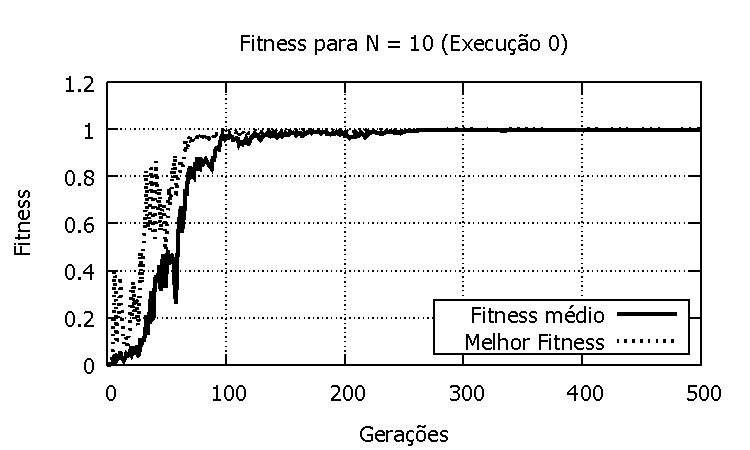
\includegraphics[width=0.48\textwidth]{figs/resultados/fitnessEL/N-10_E-0_fitness.pdf}
			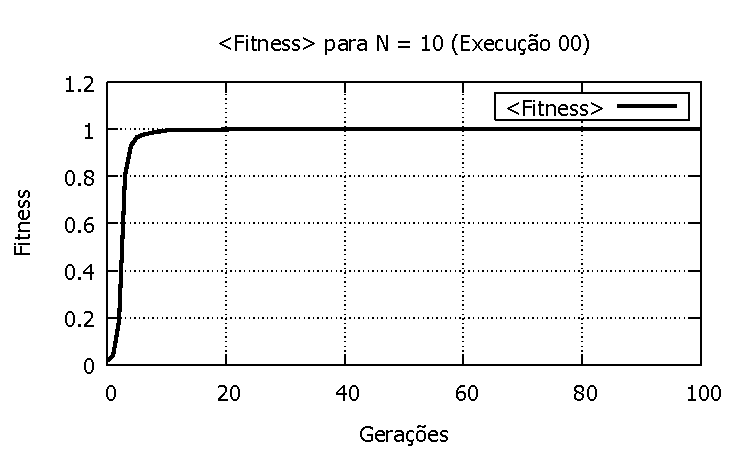
\includegraphics[width=0.48\textwidth]{figs/resultados/fitnessGrad/N10_00_fitness.pdf}
		\caption{Comportamento do \textit{fitness} para as execuções zero do Hamiltoniano de ordem 10, semente 1445738835. A primeira usa o \textit{fitness} $f_i = e^{-\lambda(\rho_i - E_L)^2}$, que chega ao autovalor mínimo, enquanto a segunda utiliza o $f_i = e^{-\lambda \| \nabla \rho_i \|^2}$.}
		\label{fig:N-10_E-0_fitness}
	\end{figure}
	
	De todo modo, as duas execuções estão conectadas pois, como partiram da mesma semente de números pseudoaleatórios, a população inicial foi \textit{exatamente} a mesma. Inclusive, na primeira geração, em ambas as execuções, os valores para $<\rho>$ e para o melhor $\rho$ foram, respectivamente, $9,876075$ e $9,557892$, igualmente distantes do autovalor mínimo $E_0 = 0,386075$. Os gráficos da figura \ref{fig:N-10_E-0_rho_comparacao} permitem comparar a evolução do $<\rho>$ nos dois casos. Assim como na figura anterior, a imagem da esquerda refere-se ao uso do \textit{fitness} $f_i = e^{-\lambda(\rho_i - E_L)^2}$.
	
	É tentador afirmar que a causa de uma execução ter sido mais lenta do que a outra foi porque percorreu um caminho mais longo ao sair de $<\rho> = 9,876075$, passar por $E_1 = 2,461056$ e continuar até encontrar $E_0 = 0,386075$, enquanto a mais rápida saiu do mesmo $<\rho>$ e parou logo que encontrou $E_1$. Infelizmente essa conclusão estaria incorreta. A maneira como os Algoritmos Genéticos viajam no espaço de soluções tem forte base estocástica e, portanto, qualquer comparação linear é extremamente arriscada, quiçá impossível. Objetivamente, posso apenas concluir que os valores finais encontrados por cada \textit{fitness} estão condizentes com a construção de cada função objetivo: $\nabla \rho_i$ leva a qualquer autovalor; $\rho_i - E_L$ encontra o autovalor mínimo.
	
	
	\begin{figure}[htbp]
		\centering
			\includegraphics[width=0.48\textwidth]{figs/resultados/fitnessEL/N-10_E-0_rho.pdf}
			\includegraphics[width=0.48\textwidth]{figs/resultados/fitnessGrad/N10_00_rho.pdf}
		\caption{Comportamento do $\rho$ para as execuções zero do Hamiltoniano de ordem 10, semente 1445738835. A primeira usa o \textit{fitness} $f_i = e^{-\lambda(\rho_i - E_L)^2}$, que chega ao autovalor mínimo, enquanto a segunda utiliza o $f_i = e^{-\lambda \| \nabla \rho_i \|^2}$.}
		\label{fig:N-10_E-0_rho_comparacao}
	\end{figure}
	
	\begin{figure}[phtb]
	\centering
  \begin{tabular}{@{}cc@{}}
    \includegraphics[width=.40\textwidth]{figs/resultados/fitnessEL/N-10_E-0_fitness-extendido.pdf} &
    \includegraphics[width=.40\textwidth]{figs/resultados/fitnessEL/N-10_E-0_rho_extendido.pdf}   \\
		\includegraphics[width=.40\textwidth]{figs/resultados/fitnessEL/N-10_E-1_fitness-extendido.pdf} &
    \includegraphics[width=.40\textwidth]{figs/resultados/fitnessEL/N-10_E-1_rho_extendido.pdf}   \\
		\includegraphics[width=.40\textwidth]{figs/resultados/fitnessEL/N-10_E-2_fitness-extendido.pdf} &
    \includegraphics[width=.40\textwidth]{figs/resultados/fitnessEL/N-10_E-2_rho_extendido.pdf}   \\
		\includegraphics[width=.40\textwidth]{figs/resultados/fitnessEL/N-10_E-3_fitness-extendido.pdf} &
    \includegraphics[width=.40\textwidth]{figs/resultados/fitnessEL/N-10_E-3_rho_extendido.pdf}   \\
		\includegraphics[width=.40\textwidth]{figs/resultados/fitnessEL/N-10_E-4_fitness-extendido.pdf} &
    \includegraphics[width=.40\textwidth]{figs/resultados/fitnessEL/N-10_E-4_rho_extendido.pdf} \\
		\includegraphics[width=.40\textwidth]{figs/resultados/fitnessEL/N-10_E-5_fitness-extendido.pdf} &
    \includegraphics[width=.40\textwidth]{figs/resultados/fitnessEL/N-10_E-5_rho_extendido.pdf}
  \end{tabular}
  \caption{Execuções para N = 10 com o \textit{fitness} $f_i = e^{-\lambda(\rho_i - E_L)^2}$.}
	\label{fig:execucoes_N10_EL}
	\end{figure}
	
	\begin{figure}[phtb]
	\centering
  \begin{tabular}{@{}cc@{}}
		\includegraphics[width=.40\textwidth]{figs/resultados/fitnessEL/N-20_E-1_fitness-extendido.pdf} &
    \includegraphics[width=.40\textwidth]{figs/resultados/fitnessEL/N-20_E-1_rho_extendido.pdf}   \\
		\includegraphics[width=.40\textwidth]{figs/resultados/fitnessEL/N-20_E-2_fitness-extendido.pdf} &
    \includegraphics[width=.40\textwidth]{figs/resultados/fitnessEL/N-20_E-2_rho_extendido.pdf}   \\
		\includegraphics[width=.40\textwidth]{figs/resultados/fitnessEL/N-20_E-3_fitness-extendido.pdf} &
    \includegraphics[width=.40\textwidth]{figs/resultados/fitnessEL/N-20_E-3_rho_extendido.pdf}   \\
		\includegraphics[width=.40\textwidth]{figs/resultados/fitnessEL/N-20_E-4_fitness-extendido.pdf} &
    \includegraphics[width=.40\textwidth]{figs/resultados/fitnessEL/N-20_E-4_rho_extendido.pdf} \\
		\includegraphics[width=.40\textwidth]{figs/resultados/fitnessEL/N-20_E-5_fitness-extendido.pdf} &
    \includegraphics[width=.40\textwidth]{figs/resultados/fitnessEL/N-20_E-5_rho_extendido.pdf}
  \end{tabular}
  \caption{Execuções para N = 20 com o \textit{fitness} $f_i = e^{-\lambda(\rho_i - E_L)^2}$.}
	\label{fig:execucoes_N20_EL}
	\end{figure}
	
	\begin{figure}[phtb]
	\centering
  \begin{tabular}{@{}cc@{}}
		\includegraphics[width=.40\textwidth]{figs/resultados/fitnessEL/N-30_E-1_fitness-extendido.pdf} &
    \includegraphics[width=.40\textwidth]{figs/resultados/fitnessEL/N-30_E-1_rho_extendido.pdf}   \\
		\includegraphics[width=.40\textwidth]{figs/resultados/fitnessEL/N-30_E-2_fitness-extendido.pdf} &
    \includegraphics[width=.40\textwidth]{figs/resultados/fitnessEL/N-30_E-2_rho_extendido.pdf}   \\
		\includegraphics[width=.40\textwidth]{figs/resultados/fitnessEL/N-30_E-3_fitness-extendido.pdf} &
    \includegraphics[width=.40\textwidth]{figs/resultados/fitnessEL/N-30_E-3_rho_extendido.pdf}   \\
		\includegraphics[width=.40\textwidth]{figs/resultados/fitnessEL/N-30_E-4_fitness-extendido.pdf} &
    \includegraphics[width=.40\textwidth]{figs/resultados/fitnessEL/N-30_E-4_rho_extendido.pdf} \\
		\includegraphics[width=.40\textwidth]{figs/resultados/fitnessEL/N-30_E-5_fitness-extendido.pdf} &
    \includegraphics[width=.40\textwidth]{figs/resultados/fitnessEL/N-30_E-5_rho_extendido.pdf}
  \end{tabular}
  \caption{Execuções para N = 30 com o \textit{fitness} $f_i = e^{-\lambda(\rho_i - E_L)^2}$.}
	\label{fig:execucoes_N30_EL}
	\end{figure}
	
	\begin{figure}[phtb]
	\centering
  \begin{tabular}{@{}cc@{}}
		\includegraphics[width=.40\textwidth]{figs/resultados/fitnessEL/N-40_E-1_fitness-extendido.pdf} &
    \includegraphics[width=.40\textwidth]{figs/resultados/fitnessEL/N-40_E-1_rho_extendido.pdf}   \\
		\includegraphics[width=.40\textwidth]{figs/resultados/fitnessEL/N-40_E-2_fitness-extendido.pdf} &
    \includegraphics[width=.40\textwidth]{figs/resultados/fitnessEL/N-40_E-2_rho_extendido.pdf}   \\
		\includegraphics[width=.40\textwidth]{figs/resultados/fitnessEL/N-40_E-3_fitness-extendido.pdf} &
    \includegraphics[width=.40\textwidth]{figs/resultados/fitnessEL/N-40_E-3_rho_extendido.pdf}   \\
		\includegraphics[width=.40\textwidth]{figs/resultados/fitnessEL/N-40_E-4_fitness-extendido.pdf} &
    \includegraphics[width=.40\textwidth]{figs/resultados/fitnessEL/N-40_E-4_rho_extendido.pdf}		\\
		\includegraphics[width=.40\textwidth]{figs/resultados/fitnessEL/N-40_E-5_fitness-extendido.pdf} &
    \includegraphics[width=.40\textwidth]{figs/resultados/fitnessEL/N-40_E-5_rho_extendido.pdf}
  \end{tabular}
  \caption{Execuções para N = 40 com o \textit{fitness} $f_i = e^{-\lambda(\rho_i - E_L)^2}$.}
	\label{fig:execucoes_N40_EL}
	\end{figure}
	
	Escolher um para discutir.
	
	Exemplos de execução:
	
	
	\begin{enumerate}
		\item \textbf{O que acontece quando $\rho_0$ está um pouco acima de $E_0$?}
		
				Para com $<\rho> \approx \rho_0$
				
				Não encontra o menor autovalor ($E_0$).
				
				Porém, verifica-se que o $<\nabla \rho> \approx 0$.
				
				Então, estamos próximos ao menor autovalor.

				
		\item \textbf{O que acontece quando $\rho_0$ está um pouco abaixo de $\lambda_0$}
						
				Encontra uma aproximação para o autovalor mínimo ($\lambda_0$).
				
				$<fitness>$ é próximo a 1 pois $<\rho>$ é próximo de $\rho_0$.
				
				$<\nabla \rho> \approx 0$.
				
						
		\item \textbf{O que acontece quando $\rho_0$ está muito acima de $E_0$?}
		
					Acredito que não encontrará uma aproximação para $E_0$, pois a região de busca está muito distante. (verificar)
					
				Para com $<\rho> \approx \rho_0$
				
				Verifica-se que o $\nabla \rho >> 0$. Portanto, estamos distantes do menor autovalor.
						
		\item \textbf{O que acontece quando $\rho_0$ está muito abaixo de $E_0$?}
				
				Acredito que não encontrará uma aproximação para $E_0$, pois a região de busca está muito distante.
				
				Para com $<\rho> \approx \rho_0$
				
				Verifica-se que o $\nabla \rho >> 0$. Portanto, estamos distantes do menor autovalor.
		
	\end{enumerate}
	
	Citar brevemente a relação entre a dificuldade (parece uma inércia) de melhorar a precisão dos resultados no final, dizer que isso está relacionado com o formato da função \textit{fitness}.

	\section{$f_i = e^{-\lambda(\rho_i - \rho_0)^2}$ leva ao autovalor mínimo ($E_0$), mas devemos saber aproximadamente onde ele está}
	
	
	Ponte para a discussão do erro \textit{fitness}
	
	\section{$f_i = e^{[-\lambda \nabla \rho]}$ é mais rápido do que $f_i = e^{[-\lambda (\nabla \rho)^2]}$}
	
	Como um dos critérios de parada utiliza $\nabla \rho$ (sem quadrado), testamos essa forma no fitness.
	
	Várias execuções.
	
	Gráfico comparando o comportamento (um termina mais rápido)
	
	Tabela com os detalhes explícitos do do ganho.
	
	Ponte pra falar sobre o outro fitness que encontra o mínimo.
	
	
\section{$f_i = e^{-\lambda(\rho_i - \rho_0)^2}$ próximo de $\rho$ é intrinsicamente impreciso}
	
	Como $\lambda$ e $\rho_0$ são constantes por definição, $f_i$ é uma função apenas de $\rho$.
	
	Função simétrica em torno de $\rho_0$.
	
	Gráfico com diferentes $\rho_0$'s para o domínio $\rho = [-200,200]$. 
	
	Para uma dada função $fitness$, em torno de zero, por exemplo, dar um \textit{zoom} no pico.
	
	\begin{figure}[htbp]
		\centering
			\includegraphics{figs/varios-fit-mono-zoom.pdf}
		\caption{Zoom próximo do pico}
		\label{fig:varios-fit-mono-zoom}
	\end{figure}
	
	
	Gráficos com $\rho = [-5,5]$ e $\rho = [-0.1,+0.1]$.
	
	Verificar que no último gráfico o SciLab já apresenta dificuldades para diferenciar os pontos de $f$.
	
	Gráfico da variação do fitness como função da variação do $\rho$ (a derivada).
	
	A derivada é 
	
	$$
		\frac{df}{d\rho} = -2\lambda(\rho - \rho0)e^{-\lambda(\rho - \rho0)^2}
	$$
	
	Com $\rho = [-200,200]$, gráfico da derivada.
	
	Gráfico comparando $f$ com $df/d\rho$. Verificar visualmente que $df/d\rho$ é muito pequeno, próximo de zero. 
	
	Tabela com os valores mostrando que, próximo à $\rho_0$, uma mudança de $\Delta\rho = 0.1$ leva a uma variação de $\Delta f <= 0.000001$.
	
	Para o algoritmo genético isso é ruim. Cada rho está associado a um indivíduo e o fitness deve diferenciar cada um, de modo que a maior nota é dada ao indivíduo mais próximo da solução.
	
	Veja que para $\rho = [-0.3,+0.3]$ o fitness é igual a 1. Nessa região a o fitness falha na diferenciação dos indivíduos.
	
	Para fitness muito pequeno há o mesmo problema. Com isso, pode-se definir uma região do fitness onde a função é apropriada para o uso dos algoritmos genéticos. Figura \ref{fig:fitness_boaRegiao}.
	
	Para Futuro, continuação do trabalho: há alguma maneira de lidar com os parâmetros de $f$ de modo a ficarmos sempre na região boa?
	
	Região boa: entre as duas linhas, quase linear.
		
	\begin{figure}[htbp]
		\centering
			\includegraphics[width=0.90\textwidth]{figs/resultados/fitness_boaRegiao.pdf}
		\caption{Boa região para o fitness (entre as duas linhas)}
		\label{fig:fitness_boaRegiao}
	\end{figure}
	
	Há um limite de precisão intrínseco com o uso desse fitness.
	
	Por isso a dificuldade em melhorar a precisão.
	
	% Table generated by Excel2LaTeX from sheet 'Plan2'
\begin{tabular}{rr}

       \textit{rho} &          \textit{f} \\

      -0,1 &   0,999996 \\

     -0,09 &   0,999997 \\

     -0,08 &   0,999997 \\

     -0,07 &   0,999998 \\

     -0,06 &   0,999999 \\

     -0,05 &   0,999999 \\

     -0,04 &   0,999999 \\

     -0,03 &          1 \\

     -0,02 &          1 \\

     -0,01 &          1 \\

         0 &          1 \\

      0,01 &          1 \\

      0,02 &          1 \\

      0,03 &          1 \\

      0,04 &   0,999999 \\

      0,05 &   0,999999 \\

      0,06 &   0,999999 \\

      0,07 &   0,999998 \\

      0,08 &   0,999997 \\

      0,09 &   0,999997 \\

       0,1 &   0,999996 \\

\end{tabular}  

		
		O parâmetro $\lambda$ também influencia fortemente o fitness e o algoritmo genético.
		
		Ponte para a discussão do $\lambda$.
		
	\section{Por que o $\lambda$ deve ser escolhido cuidadosamente?}
	
	Execuções para N=10 com diferentes $\lambda$'s. Com os gráficos, explicar o que o artigo de 2004 quis dizer com \textit{fitness overflow/underflow}.
	
	Gráficos com rho entre 0 e 250 (exemplo pra N=10), mas com cortes em diferentes rhos.
	
	\begin{figure}[pt]
	\centering
		\includegraphics{figs/varios-fits-color.pdf}
	\caption{Fitness em função do lambda $-$ colorido}
	\label{fig:varios-fits-color}
\end{figure}

\begin{figure}[pb]
	\centering
		\includegraphics{figs/varios-fits-mono.pdf}
	\caption{Fitness em função do lambda}
	\label{fig:varios-fits-mono}
\end{figure}

	Explicar que uma boa escolha do $\lambda$ deve cobrir todos os autovalores. Citar as execuções anteriores (boas e ruins em função de cada $\lambda$).
	
	Gráfico com $\lambda$ fazendo o fitness cortar em um $\rho$ muito baixo. Discutir puxando as execuções anteriores.
	
	Outro gráfico, mas com $\lambda$ fazendo o fitness cortar em um $\rho$ muito alto. Discutir puxando as execuções anteriores.
	
	Gráfico com uma boa escolha de $\lambda$. Discutir puxando as execuções anteriores.
	
	Após estimativa, refinar a obtenção do $\lambda$. Alterar o $lambda$ (valores em torno da estimativa), executar o programa para verificar se o fitness médio da primeira população é baixo. (se a população inicial tem fitness muito grande, há convergência prematura).
	
	Tabela com alguns $lambdas$ encontrados dessa maneira (estimativa e refinamento).
	
	Infelizmente, para cada matriz, um $\lambda$ diferente.
	
	Ponte pra equação empírica do $\lambda$.
	
	\section{Equação empírica para o $\lambda$}
	
	Delineamento da equação como feito na reunião de 29/09.
	
	Isolar $\lambda$ a partir da $f=e^{-\lambda*(\rho - \rho_0)^2}$
	
	Fazer $f = 0.00001 \approx 0$.
	
	Substituir $(\rho - \rho_0)^2$ por $E_{central} - E_{mínimo}$. Justificar.
	
	Regressão linear para $E_{central} - E_{mínimo}$ com função apenas da ordem da matriz (N).
	
	Inserir a Equação obtida na regressão na equação de $\lambda$.
	
	Fator $0.65$: obtido empiricamente de modo que o $\lambda$ seja semelhante aos encontrados pelo processo de estimativa e refinamento.
	
	Exemplo de execução com $\lambda$ automático.
	
	Explicitar que essa equação é válida apenas para matrizes de Coope$-$Sabo. Apesar disso, foi importante para o estudo pois permitiu automação completa.
		
	\section{A mistura de $(\rho - \rho_0)^2$ com $\nabla\rho$ não leva a melhores resultados}
	
	Como em seção anterior verificamos que $f_i = e^{[-\lambda \nabla \rho]}$ é mais rápido do que $f_i = e^{[-\lambda (\nabla \rho)]}$, e que o $\nabla\rho$ está diretamente associado aos autovalores, pensei na seguinte hipótese: inserir $\nabla \rho$ ao fitness com $(\rho - \rho_0)^2$ traria resultados mais rápidos.
	
	Justificativas para a hipótese: 
	
	\begin{enumerate}
		\item Inserir $\nabla \rho$ no fitness puniria os $\rho$'s que, apesar de próximos de $\rho_0$, não fossem autovalor. Em outras palavras, o termo $\rho - \rho_0 \approx 0$, mas $\nabla \rho >> 0$ e, portanto, o fitness ficaria pequeno.
		
		\item Como o fitness, a princípio, estaria diferenciamento melhor os bons indivíduos, o algoritmo teria uma taxa de convergência maior.
		
	\end{enumerate}
	
		Executar $10$ para o primeiro fitness, e, utilizando as mesmas dez sementes, executar outros $10$ testes com ou outro fitness.
		
		Comparação dos resultados: gráficos do comportamento do fitness e tabela comparando a velocidade de convergência (em que geração o critério de parada foi atingido), tempo de execução e erro relativo ao menor autovalor ``exato'' (obtido no SciLab).
	
	\section{Resultados preliminares na GPU}
	
		\subsection{ONEMAX na GPU}
	
				ERAD: artigo $+$ poster
				
		\subsection{Método paralelizado (versão atual, com ganho de $1,4$}
		
				Falar um pouco.
		
				